\documentclass{beamer}
\usetheme{Antibes}
% \setbeamertemplate{navigation symbols}{} 
\usefonttheme[onlymath]{serif}
\usepackage{animate}
\usepackage{amsmath}
\usepackage{lmodern}%
% \usepackage{showframe} 

\definecolor{yellow}{RGB}{255,197,051}
\definecolor{blue}  {RGB}{124,192,217}
\definecolor{green} {RGB}{139,158,119}
\definecolor{orange}{RGB}{232,099,044}
\definecolor{red}   {RGB}{219,053,038}
\definecolor{purple}{RGB}{109,110,146}

\usepackage{tikz}
\usetikzlibrary{arrows.meta}
\usetikzlibrary{calc}
\tikzstyle{block}=[rectangle,text=white,text width=5.5cm,text centered,rounded corners,minimum height=2cm]
\tikzset{
    hyperlink node/.style={
        alias=sourcenode,
        append after command={
            let     \p1 = (sourcenode.north west),
                \p2=(sourcenode.south east),
                \n1={\x2-\x1},
                \n2={\y1-\y2} in
            node [inner sep=0pt, outer sep=0pt,anchor=north west,at=(\p1)] {\hyperlink{#1}{\XeTeXLinkBox{\phantom{\rule{\n1}{\n2}}}}}
                    %xelatex needs \XeTeXLinkBox, won't create a link unless it
                    %finds text --- rules don't work without \XeTeXLinkBox.
                    %Still builds correctly with pdflatex and lualatex
        }
    }
}

\usepackage{graphicx}
\graphicspath{{.}{images/}}

\setbeamertemplate{caption}{\raggedright\insertcaption\par}

\title[Theoretical Optical Second-Harmonic Calculations for Surfaces
\hspace{5.5cm}\insertframenumber/\inserttotalframenumber]
{Theoretical Optical Second-Harmonic Calculations for Surfaces}
\author{\texorpdfstring{Sean M. Anderson\vspace{-0.7em}}{Sean M. Anderson}}
\institute{Centro de Investigaciones en \'Optica, A.C\vspace{-1em}}
\date{\small July 14, 2016\vspace{-1.2em}}
\titlegraphic{
\vspace{-3.2em}
\begin{figure}
\animategraphics[loop,scale=1.1]{12}{images/source/animation/shg-frame}{000}{058}
% 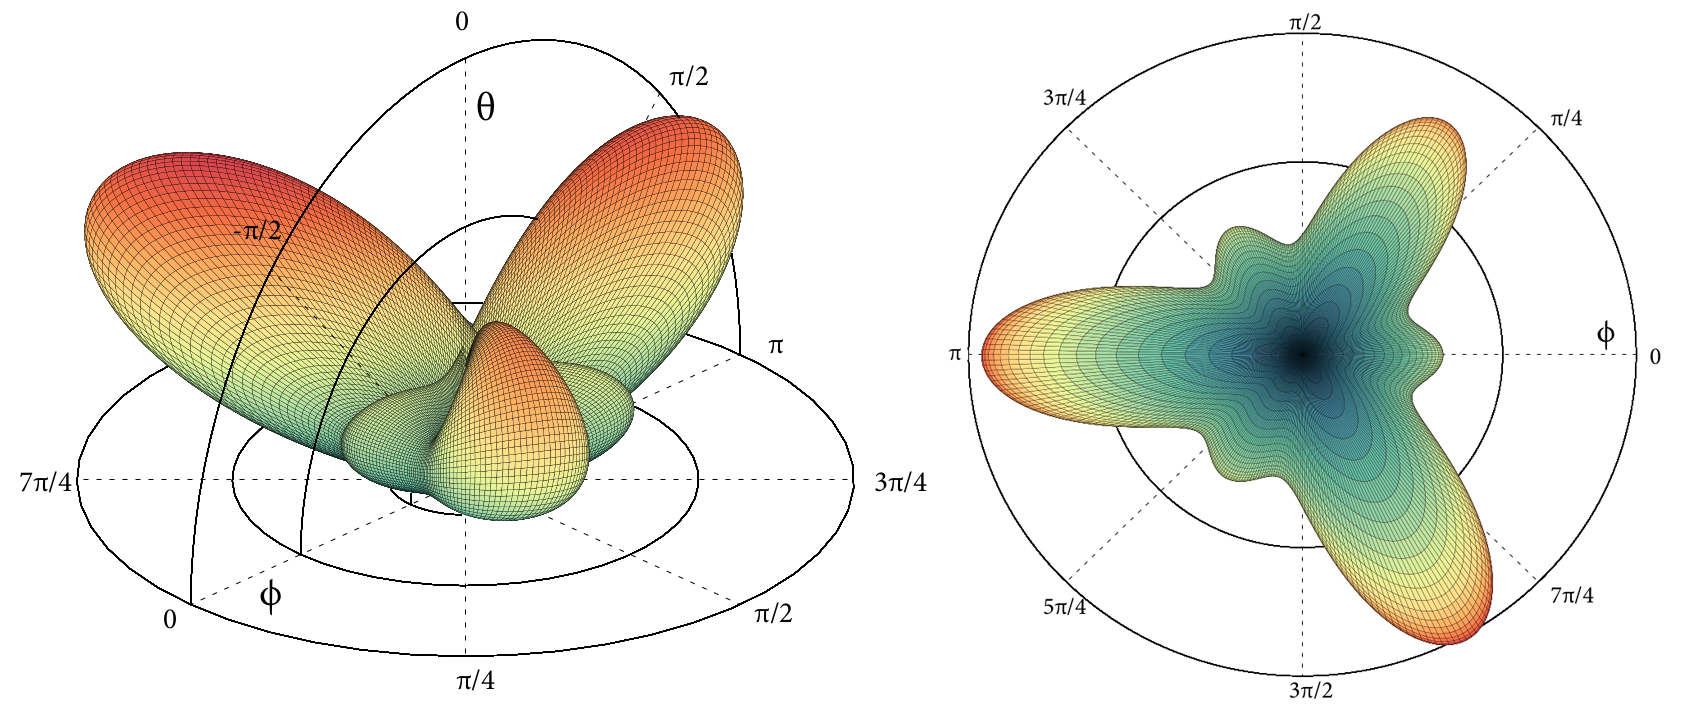
\includegraphics[width=0.8\textwidth]{3D-cover}
\end{figure}}


\begin{document}

\begin{frame}
\maketitle
\end{frame}

%%%%%%%%%%%%%%%%%%%%%%%%%%%%%%%%%%%%%%%%%%%%%%%%%%%%%%%%%%%%%%%%%%%%%%%%%%%%%%%%
%%%%%%%%%%%%%%%%%%%%%%%%%%%%%%%%%%%%%%%%%%%%%%%%%%%%%%%%%%%%%%%%%%%%%%%%%%%%%%%%

\section{Introduction}

\begin{frame}
\frametitle{Second Harmonic Generation (SHG)}
\begin{block}{Characteristics\footnote{Image: Jon Chui}}
\begin{itemize}
\item Two photons of the same frequency combine
\item Create one photon of double the frequency
\end{itemize}
\end{block}
\begin{figure}
\centering
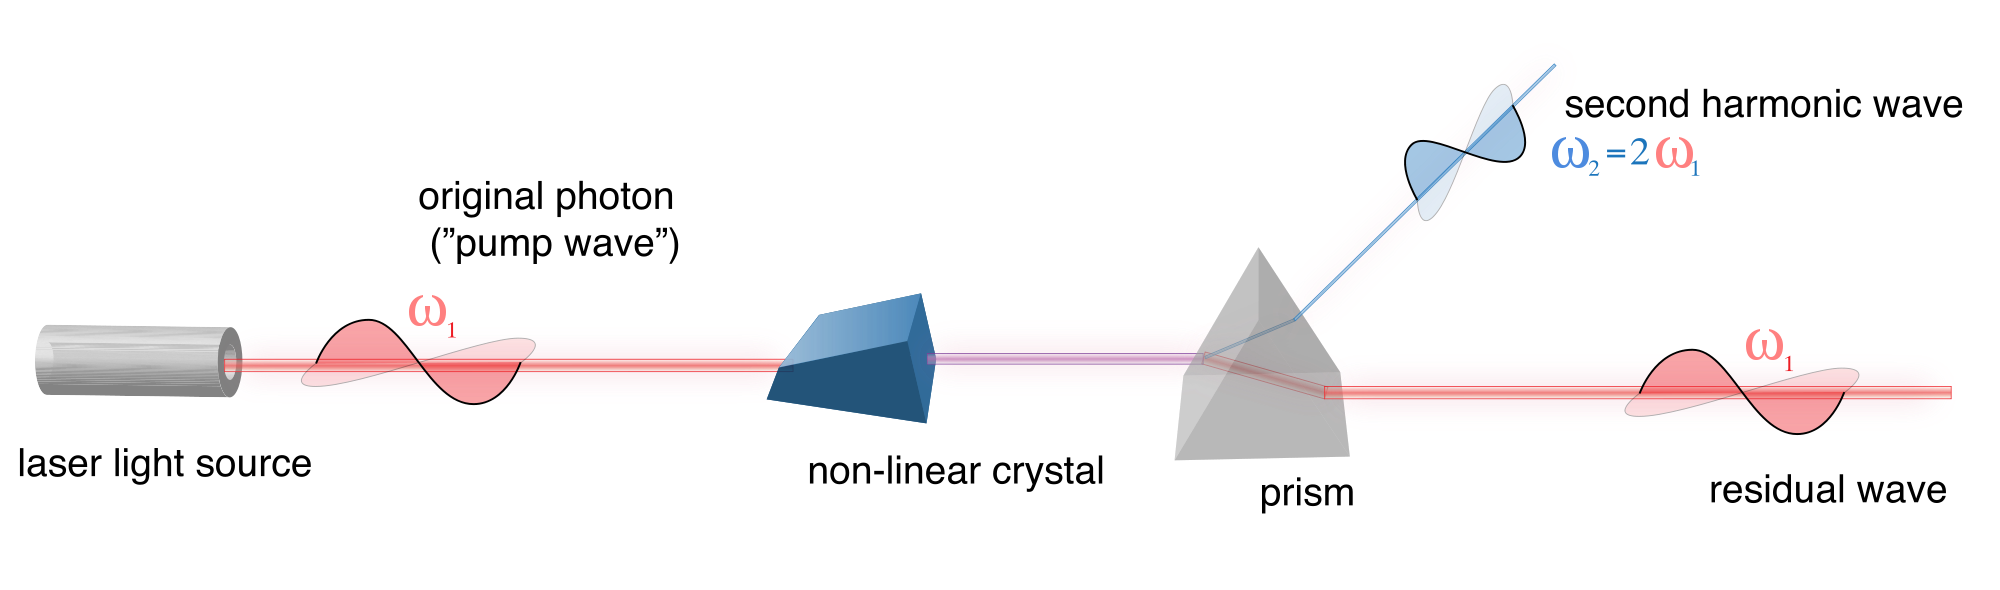
\includegraphics[width=0.9\textwidth]{diag-shg}
\end{figure}
\end{frame}

\subsection{Applications}

\begin{frame}
\frametitle{Frequency Conversion%
\footnote{Images: Dr. Ram\'on Carriles Jaimes, Cornelia Reitb\"ock}}
\begin{columns}
\column{0.5\textwidth}
\begin{figure}
\centering
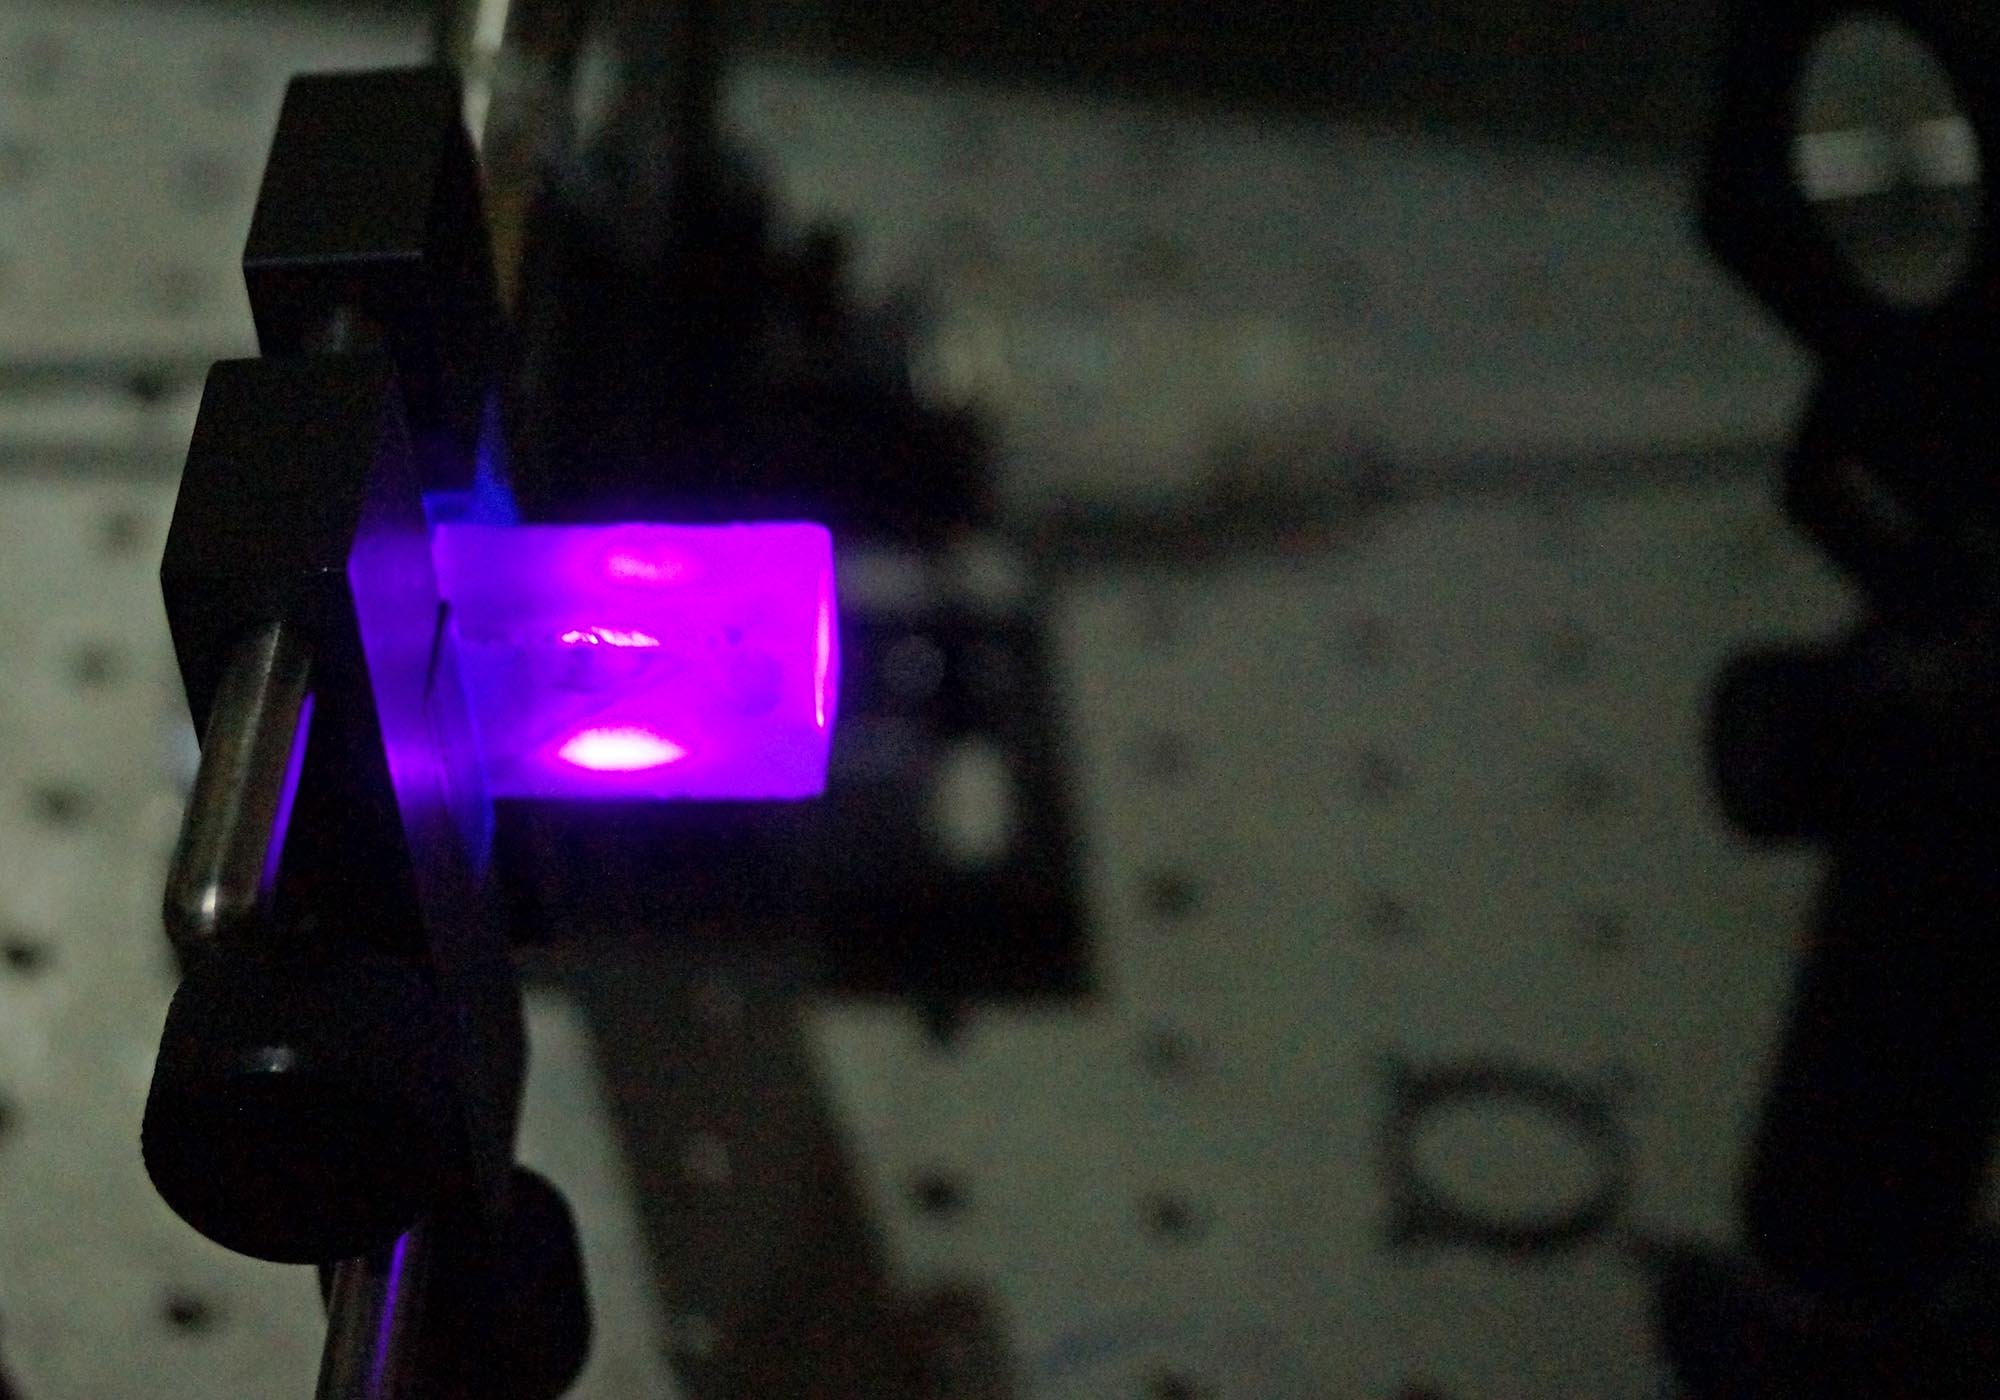
\includegraphics[width=\textwidth]{image-ramon}
\end{figure}
\column{0.5\textwidth}
\begin{figure}
\centering
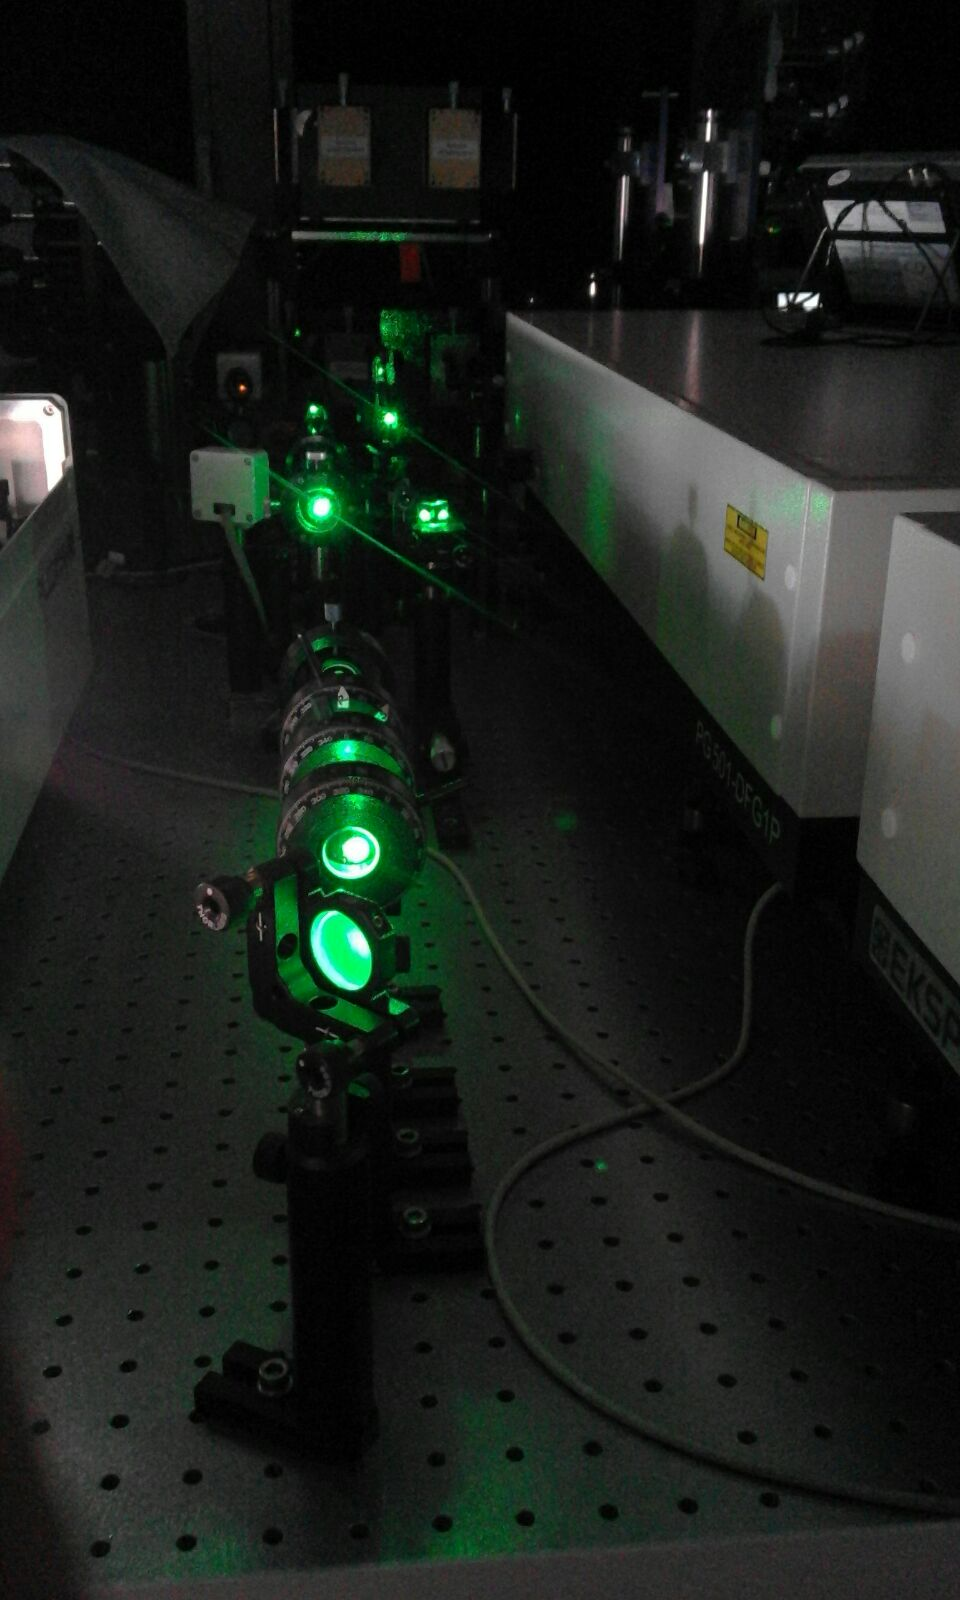
\includegraphics[height=0.7\textheight]{image-conny}
\end{figure}
\end{columns}
\end{frame}

\begin{frame}
\frametitle{Strain in TSVs%
\footnote{\emph{Cho et al.}, Appl. Phys. Lett. 108, 151602 (2016)}
\footnote{\emph{Mendoza et al.}, Phys. Status Solidi B 253, 2 (2016)}}
\begin{columns}
\column{0.5\textwidth}
\begin{figure}
\centering
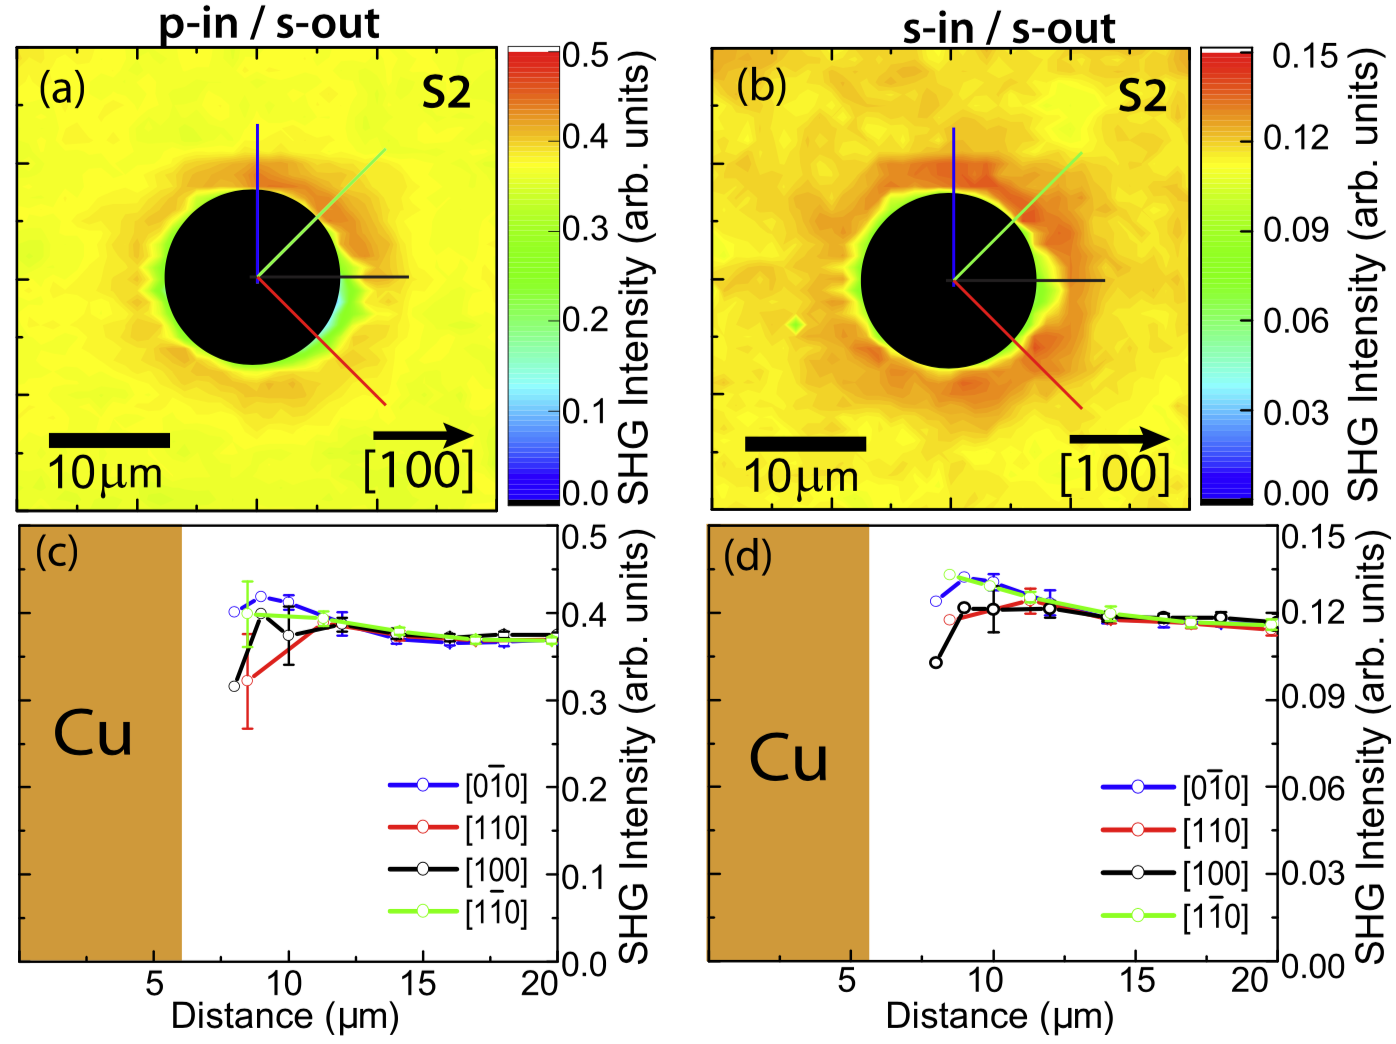
\includegraphics[width=\textwidth]{image-yojin}
\vspace*{0.5cm}
\caption{Experiment}
\end{figure}
\column{0.5\textwidth}
\begin{figure}
\centering
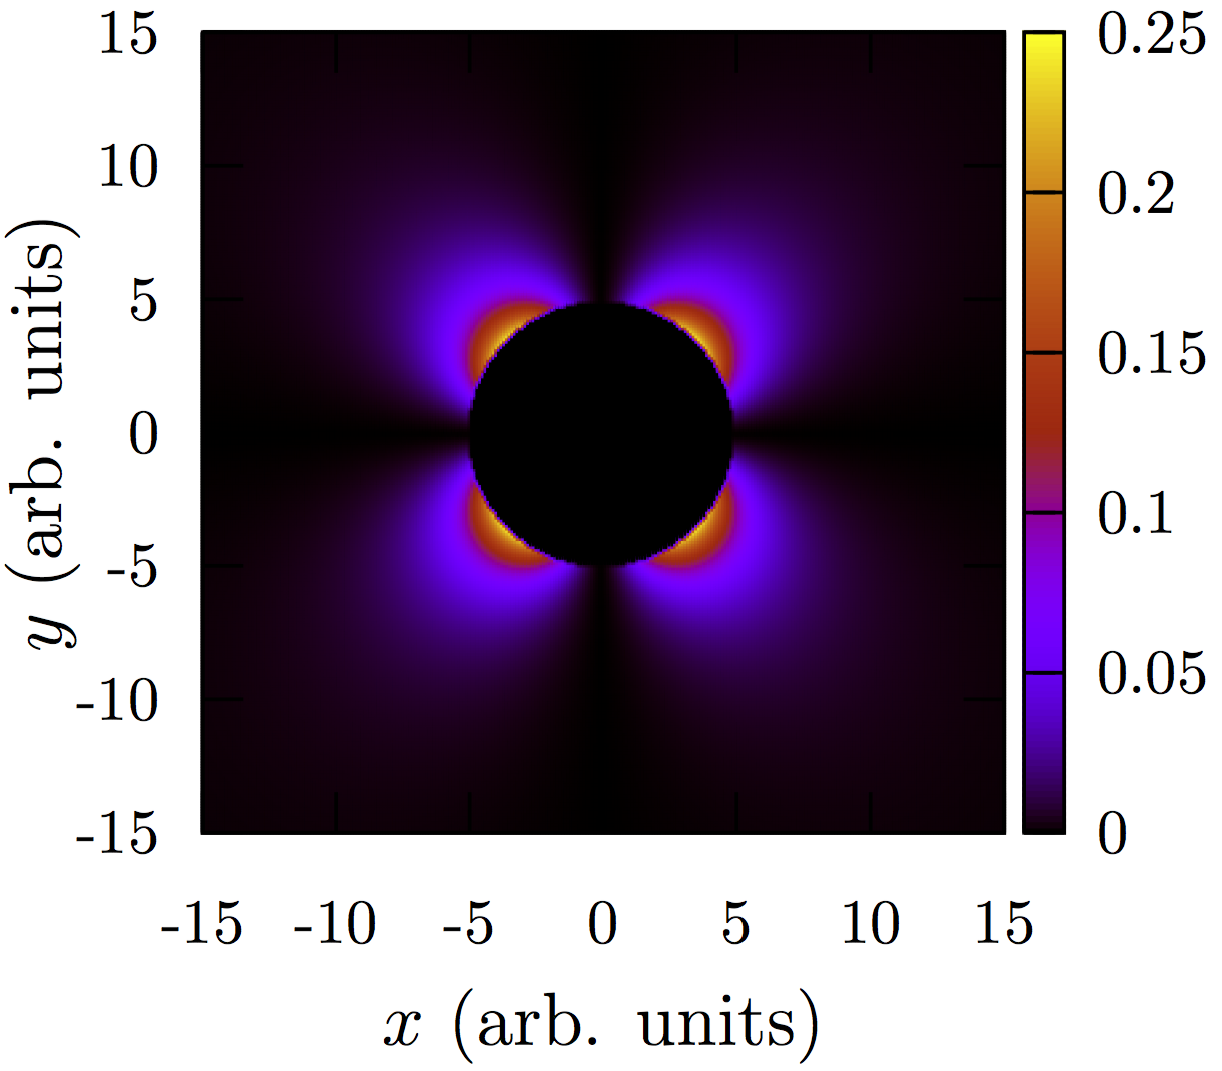
\includegraphics[width=\textwidth]{image-bms}
\caption{Theory}
\end{figure}
\end{columns}
\end{frame}

% \begin{frame}
% % \frametitle{Second Harmonic Generation (SHG)}
% \begin{columns}
% \column{0.5\textwidth}
% \begin{figure}
% \centering
% \includegraphics[width=\textwidth]{diag-levelsflourescence}
% \caption{\centering Two-photon excited fluorescence (real transitions)}
% \end{figure}
% \column{0.5\textwidth}
% \begin{figure}
\centering
% \includegraphics[width=\textwidth]{diag-levelsshg}
% \caption{\centering Second-harmonic generation\qquad(virtual transitions)}
% \end{figure}
% \end{columns}
% \end{frame}

\subsection{}

\begin{frame}
\frametitle{Second-order Nonlinear Effects}
Second-order nonlinear processes\footnote{\emph{Armstrong et al.}, Phys. Rev.
127, 1918 (1962)}
\footnote{\emph{Bloembergen et al.}, Phys. Rev. 128, 606 (1962)}
\begin{itemize}
\item Are dipole forbidden in the bulk of centrosymmetric materials
\item Are related to $\chi^{(2)}$, the nonlinear susceptibility
\item Have bigger dipolar (surface) than quadrupolar contributions
\end{itemize}\vfill
\begin{block}{Summary}
SHG is well suited for studying surfaces and interfaces!
\end{block}
\end{frame}

\begin{frame}
\frametitle{Centrosymmetric Materials}
A centrosymmetric material is a material that displays inversion symmetry, such
that $p(a,b,c) \rightarrow p(-a,-b,-c)$.
\begin{figure}
\centering
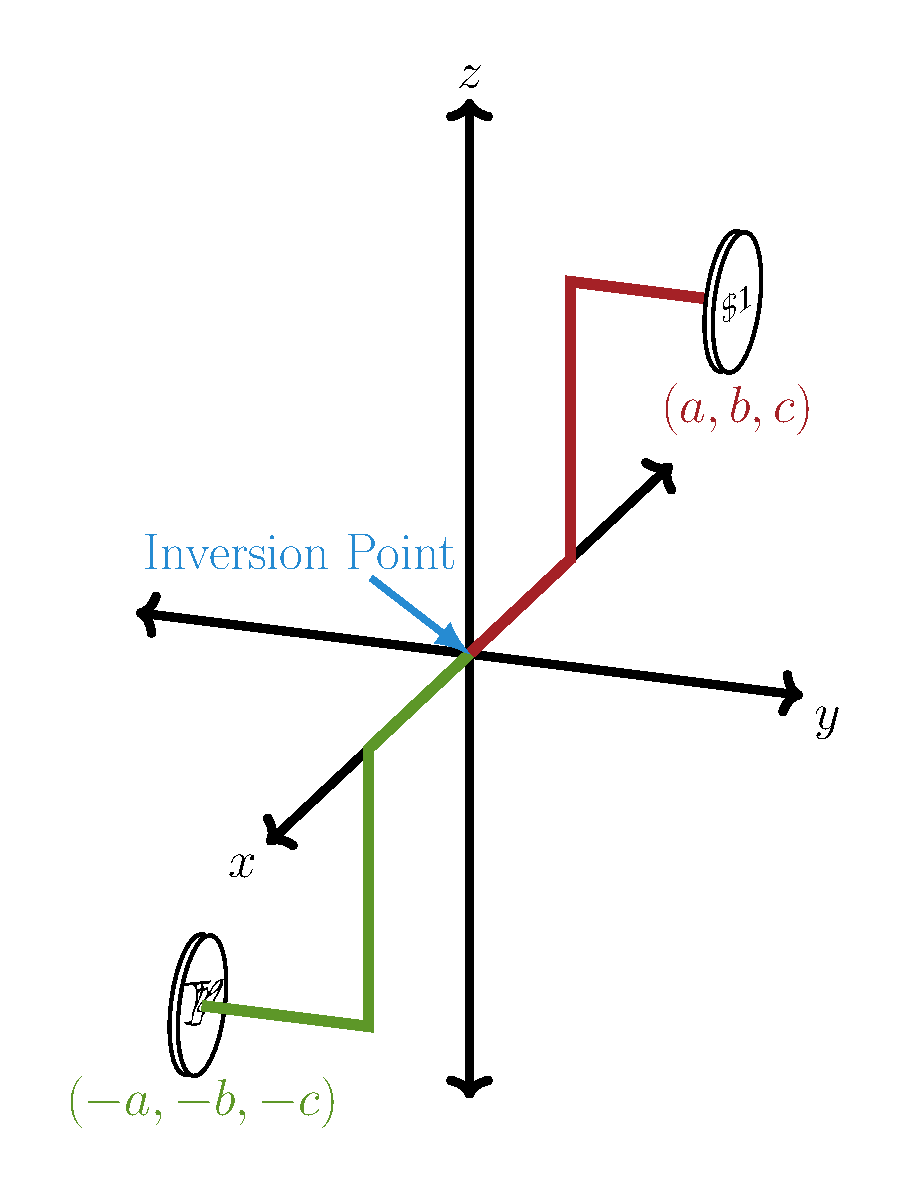
\includegraphics[height=0.7\textheight]{diag-centrosymmetry}
\end{figure}
\end{frame}

\begin{frame}
\begin{figure}
\centering
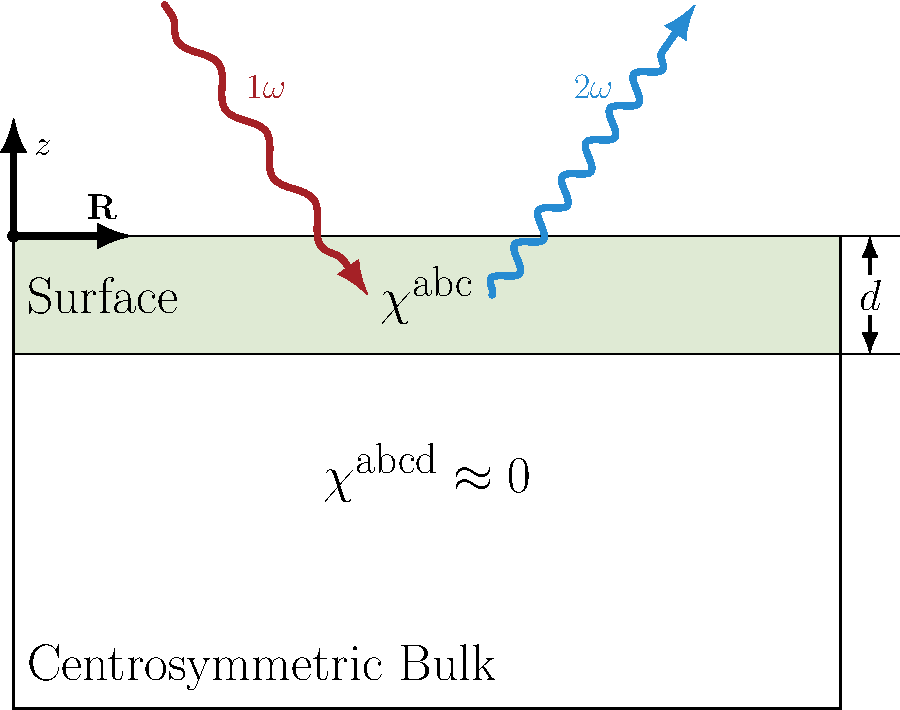
\includegraphics[width=0.8\textwidth]{diag-system}
\caption{Semi-infinite system with a centrosymmetric bulk and a surface region
is of thickness $\sim d$. Dipolar SHG is produced in reflection from the
surface.}
\end{figure}
\end{frame}

\begin{frame}
\frametitle{Two Si Test Cases}
\begin{columns}
\column{0.5\textwidth}
\begin{figure}
\centering
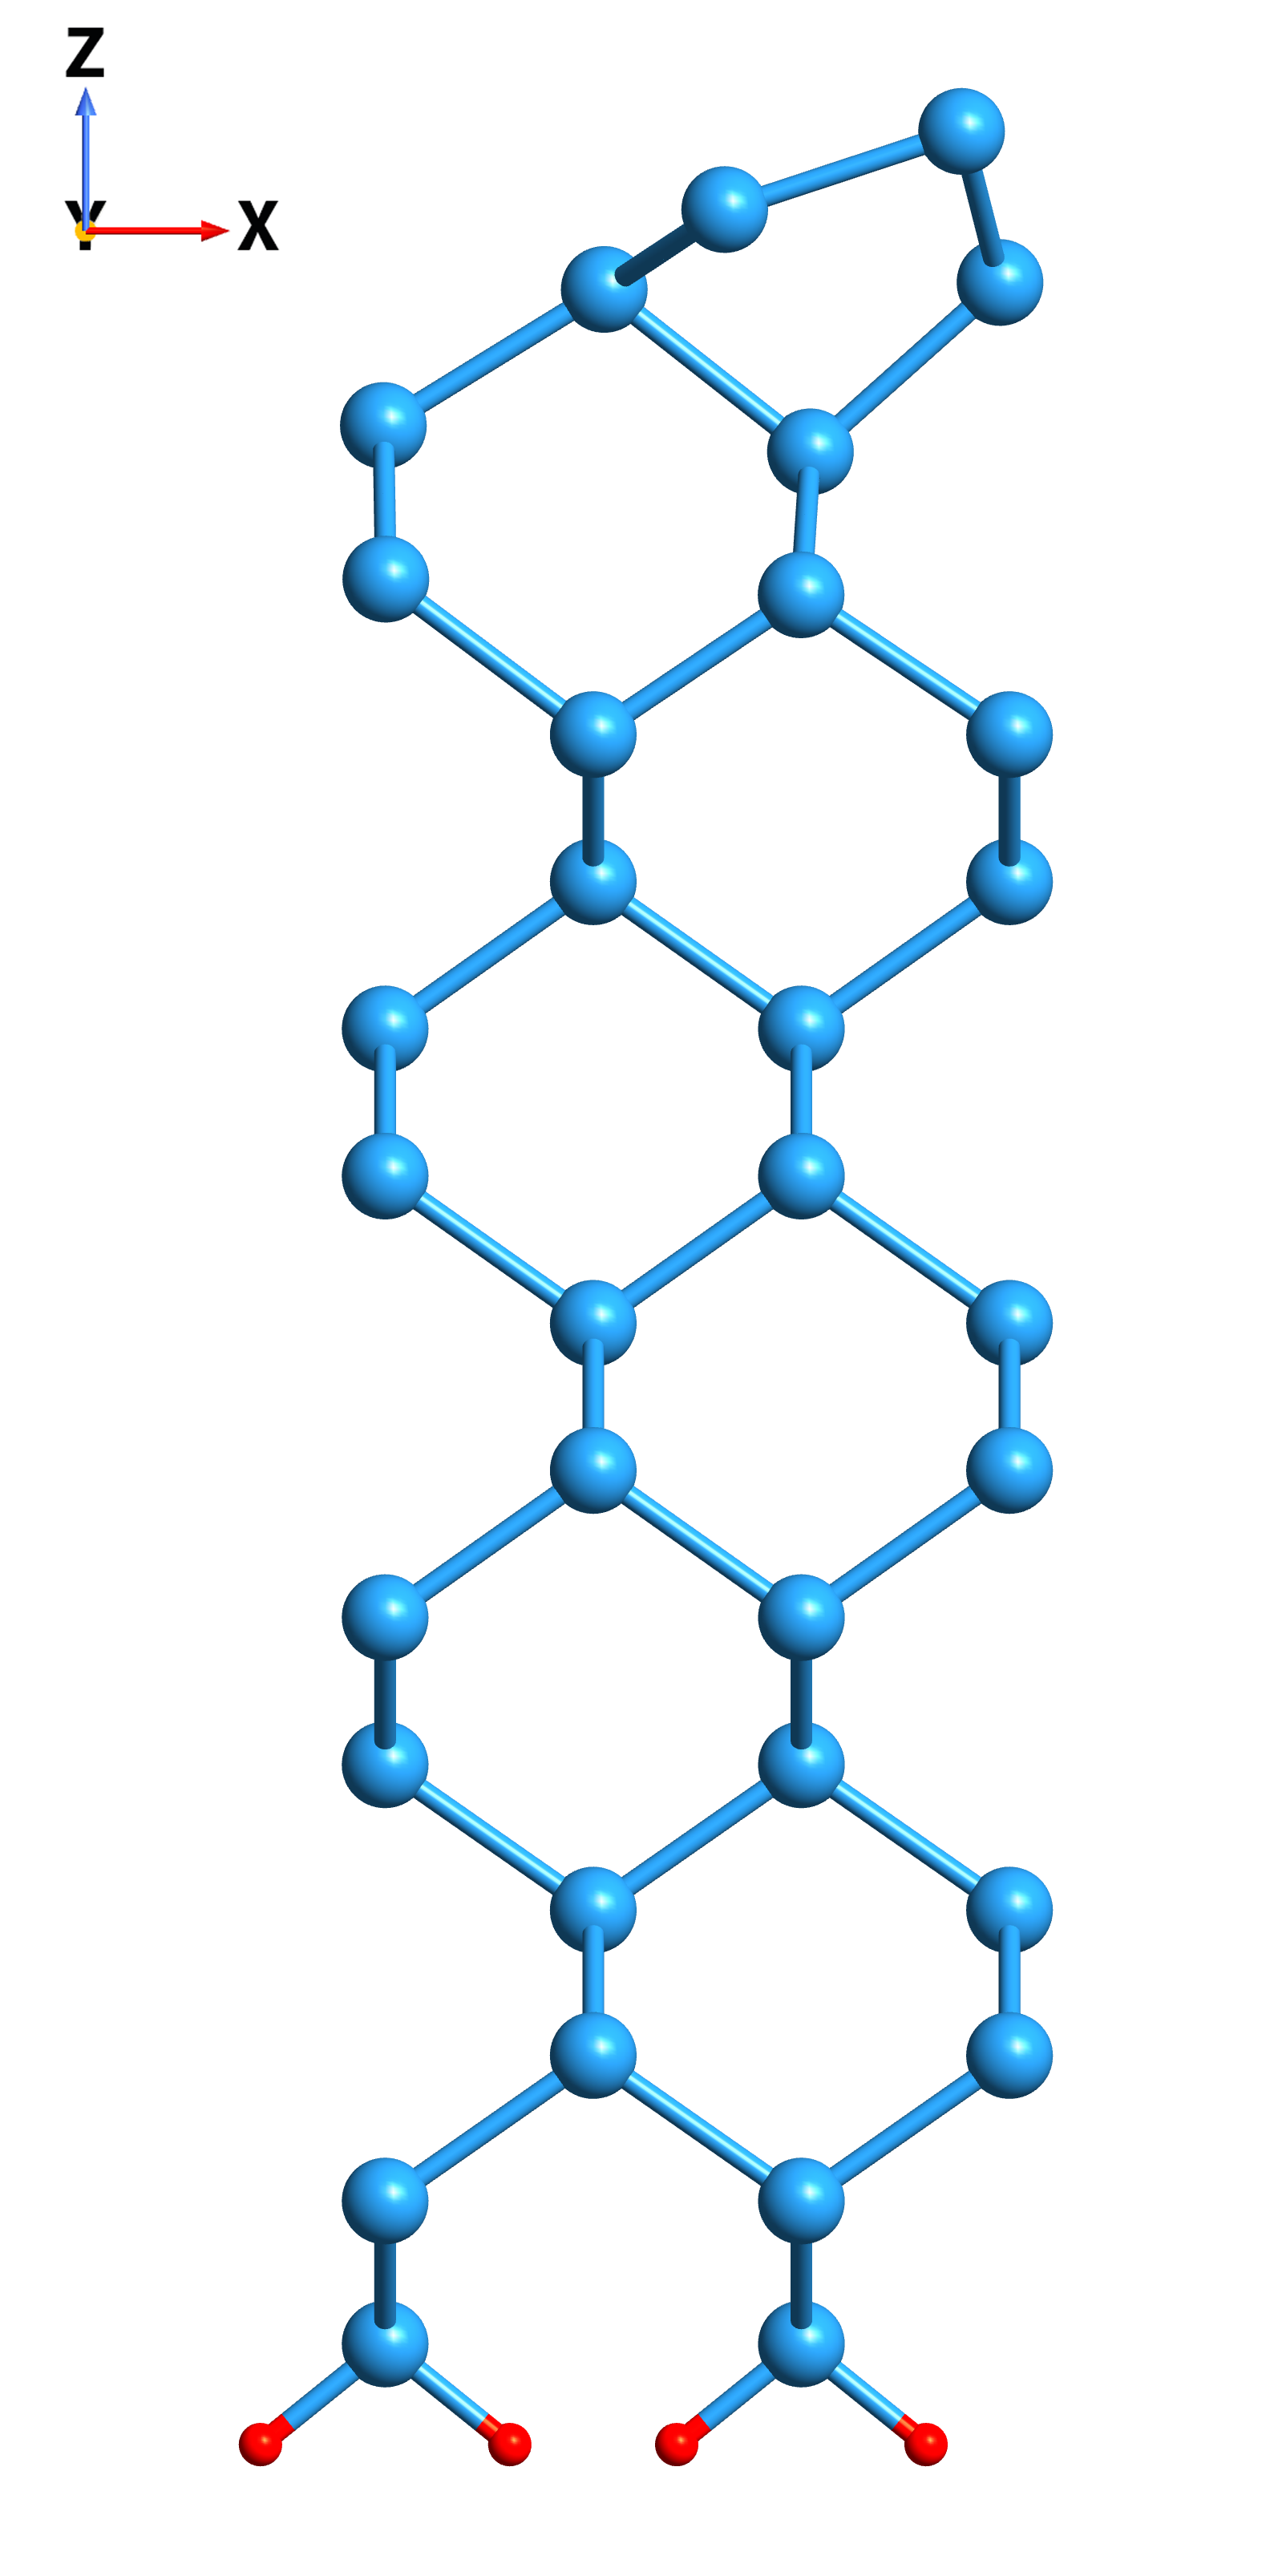
\includegraphics[height=0.7\textheight]{struc-Si2x1-front}
\vspace{-0.4cm}
\caption{Si(001)(2$\times$1)}
\end{figure}
\column{0.5\textwidth}
\begin{figure}
\centering
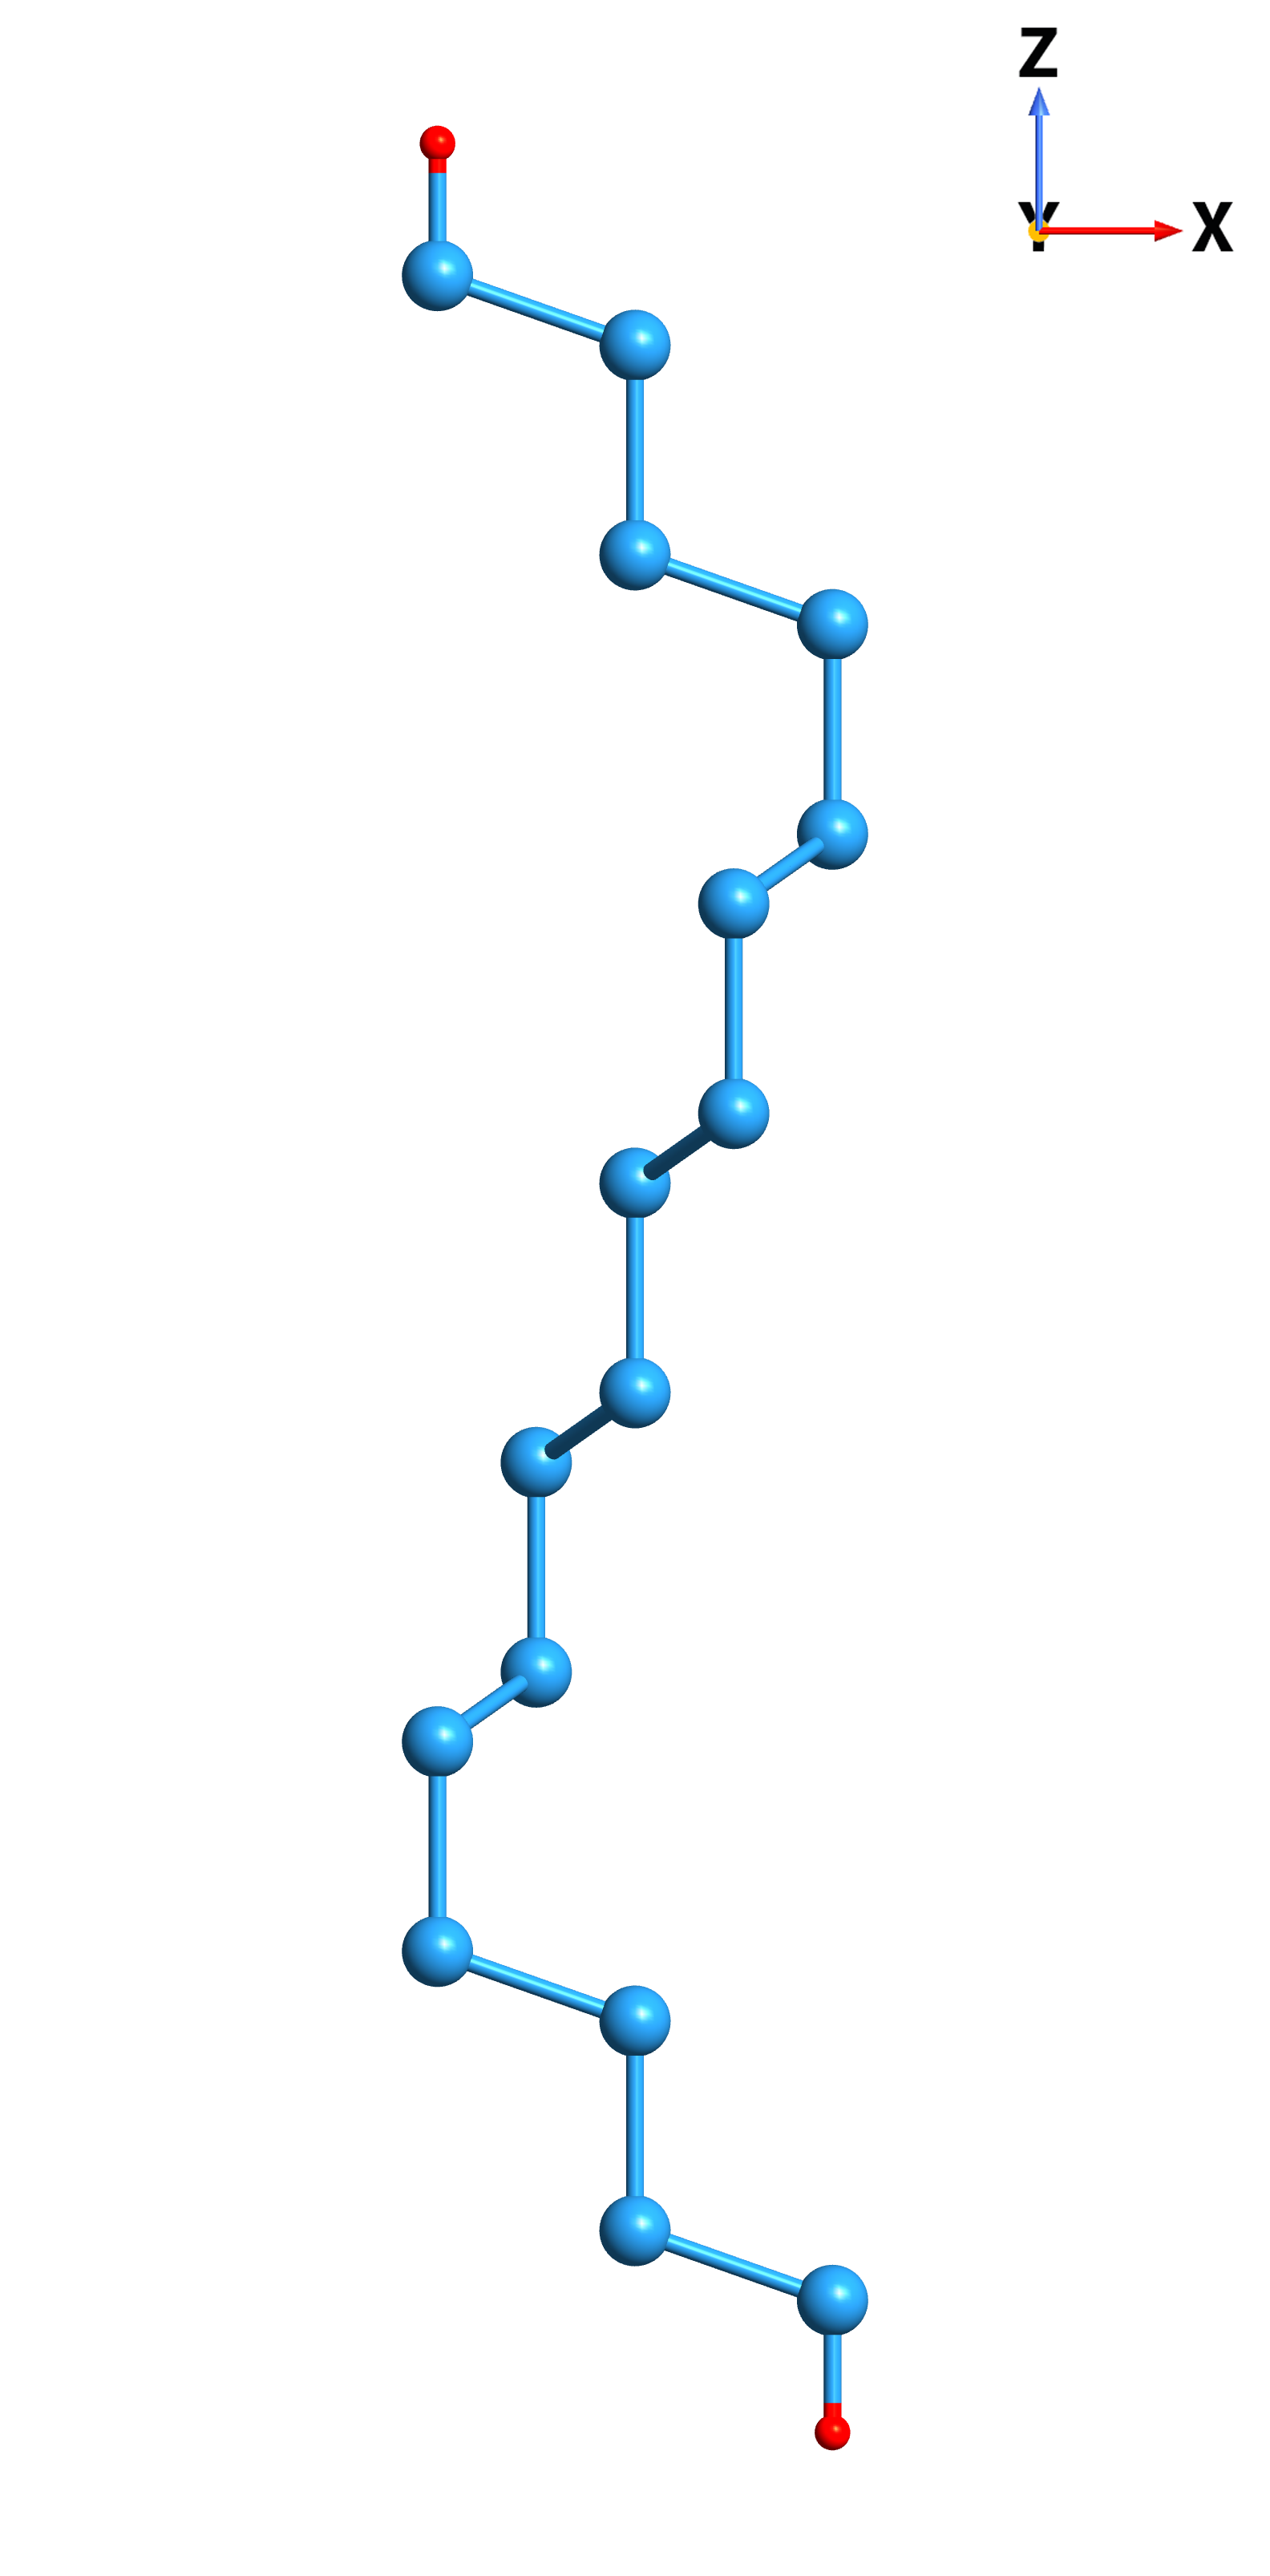
\includegraphics[height=0.7\textheight]{struc-Si1x1-front}
\vspace{-0.4cm}
\caption{Si(111)(1$\times$1):H}
\end{figure}
\end{columns}
\end{frame}


%%%%%%%%%%%%%%%%%%%%%%%%%%%%%%%%%%%%%%%%%%%%%%%%%%%%%%%%%%%%%%%%%%%%%%%%%%%%%%%%
%%%%%%%%%%%%%%%%%%%%%%%%%%%%%%%%%%%%%%%%%%%%%%%%%%%%%%%%%%%%%%%%%%%%%%%%%%%%%%%%

\section{The Nonlinear Surface Susceptibility}


%%%%%%%%%%%%%%%%%%%%%%%%%%%%%%%%%%%%%%%%%%%%%%%%%%%%%%%%%%%%%%%%%%%%%%%%%%%%%%%%

\subsection{Nonlocal Operators}

\begin{frame}
\frametitle{New Contributions to the Theory}
Our new formulation adds three contributions (within the IPA):%
\footnote{\emph{Anderson et al.}, Phys. Rev. B. 91, 075302 (2015)}
\begin{enumerate}
\item The scissors correction
\item The contribution from the nonlocal part of the pseudopotential
\item The layered cut function
\end{enumerate}
\end{frame}

\begin{frame}
\frametitle{Electron Position Operator}
We have the electron position operator as 
\begin{equation*}
\mathbf{r} = \mathbf{r}_{i} + \mathbf{r}_{e},
\end{equation*}
for interband ($e$) and intraband ($i$) transitions. The matrix elements of
$\mathbf{r}_{i}$ and $\mathbf{r}_{e}$ are given by
\begin{align*}
\langle n\mathbf{k}\vert \mathbf{r}_{i} |m\mathbf{k}'\rangle 
&= \delta_{nm}
\left[
  \delta(\mathbf{k} - \mathbf{k}')\boldsymbol{\xi}_{nn}(\mathbf{k})
+ i\nabla_{\mathbf{k}}\delta(\mathbf{k} - \mathbf{k}')
\right],\\\\
\langle n\mathbf{k}| \mathbf{r}_{e} |m\mathbf{k}'\rangle 
&= (1- \delta_{nm})\delta(\mathbf{k}-\mathbf{k}')
   \boldsymbol{\xi}_{nm}(\mathbf{k}).
\end{align*}
\end{frame}

\begin{frame}
\frametitle{Scissors Operator and
\texorpdfstring{$\mathbf{v}^{\mathrm{nl}}$}{vnl} (1 \& 2)}
We express the electron velocity operator as
\begin{equation*}\label{vop2}
\begin{split}
\mathbf{v}^{\Sigma}
&=\mathbf{v} + \mathbf{v}^{\mathrm{nl}} 
+ \mathbf{v}^{\mathcal{S}}
= \mathbf{v}^\mathrm{LDA} + \mathbf{v}^{\mathcal{S}},
\end{split}
\end{equation*}
where
\begin{equation*}\label{conhr}
\begin{split}
\mathbf{v} &=\frac{\mathbf{p}}{m_{e}},\\
\mathbf{v}^{\mathrm{nl}} &= \frac{1}{i\hbar}
  \left[\mathbf{r},V^{\mathrm{nl}}\right],\\
\mathbf{v}^{\mathcal{S}} &= \frac{1}{i\hbar}
  \left[\mathbf{r},S(\mathbf{r},\mathbf{p})\right],\\
\mathbf{v}^\mathrm{LDA} &= \mathbf{v}+\mathbf{v}^{\mathrm{nl}}.
\end{split}
\end{equation*}
We also have that
\begin{equation*}
\mathbf{r}_{nm}(\mathbf{k})
= \frac{\mathbf{v}^{\Sigma}_{nm}(\mathbf{k})}{i\omega^{\Sigma}_{nm}(\mathbf{k})}
= \frac{\mathbf{v}^{\mathrm{LDA}}_{nm}(\mathbf{k})}
       {i\omega^{\mathrm{LDA}}_{nm}(\mathbf{k})}.
\end{equation*} 
\end{frame}


%%%%%%%%%%%%%%%%%%%%%%%%%%%%%%%%%%%%%%%%%%%%%%%%%%%%%%%%%%%%%%%%%%%%%%%%%%%%%%%%

\subsection{Layered Cut Function}

\begin{frame}
\frametitle{Layered Cut Function (3)}
We introduce the cut function
\begin{equation*}
{\boldsymbol{\mathcal{C}}}(z)=\Theta(z-z_\ell+\Delta_\ell^{b})  
            \Theta(z_\ell-z+\Delta_\ell^f),
\label{sz}
\end{equation*}
that transforms any operator into its calligraphic counterpart as
\begin{equation*}
\mathbf{V} \to \boldsymbol{\mathcal{V}}
= \frac{\boldsymbol{\mathcal{C}}(z) \mathbf{V}
+ \mathbf{V} \boldsymbol{\mathcal{C}}(z)}{2},
\label{vcali}
\end{equation*} 
\end{frame}

\begin{frame}
\frametitle{Layered Cut Function (3)}
\begin{figure}
\centering
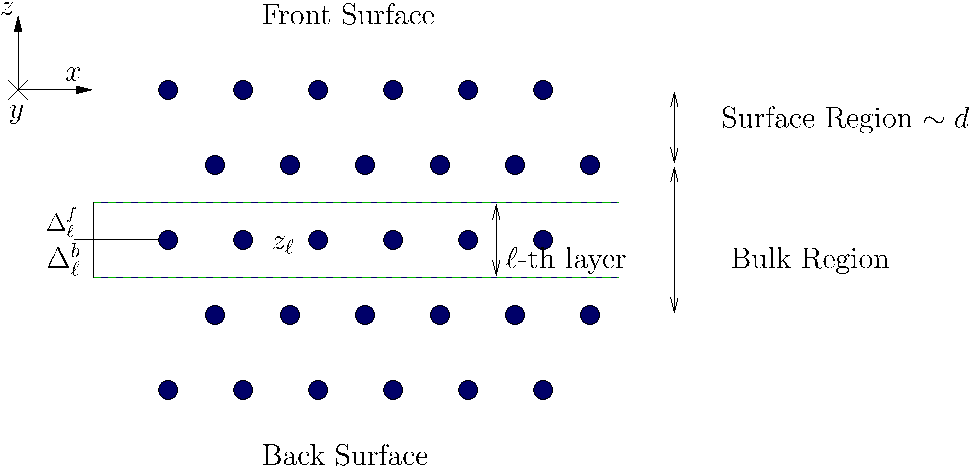
\includegraphics[width=0.9\textwidth]{diag-slab}
\caption{Sketch of the super-cell. The atomic slab corresponds to the circles
representing the atoms of the system.}
\end{figure}
\end{frame}

%%%%%%%%%%%%%%%%%%%%%%%%%%%%%%%%%%%%%%%%%%%%%%%%%%%%%%%%%%%%%%%%%%%%%%%%%%%%%%%%

\subsection{Summary}

\begin{frame}
\frametitle{Final Expressions}
\begin{block}{Interband Contribution {\tiny $\langle n\mathbf{k}|
\mathbf{r}_{e} |m\mathbf{k}'\rangle = (1- \delta_{nm})
\delta(\mathbf{k}-\mathbf{k}')\boldsymbol{\xi}_{nm}(\mathbf{k})$}}
\begin{figure}
\centering
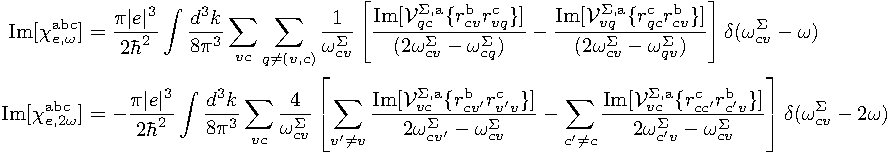
\includegraphics[scale=0.70]{chis_inter}
\end{figure}
\end{block}
\begin{alertblock}{Intraband Contribution {\tiny $\langle n\mathbf{k}\vert
\mathbf{r}_{i} |m\mathbf{k}'\rangle = \delta_{nm}
\left[\delta(\mathbf{k} - \mathbf{k}')\boldsymbol{\xi}_{nn}(\mathbf{k}) +
i\nabla_{\mathbf{k}}\delta(\mathbf{k} - \mathbf{k}')\right]$}}
\begin{figure}
\centering
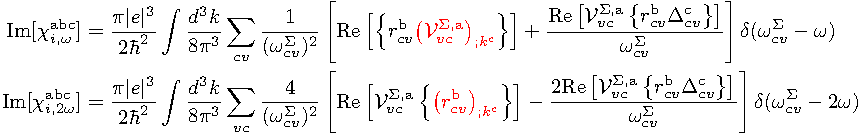
\includegraphics[scale=0.70]{chis_intra_red}
\end{figure}
\end{alertblock}
\end{frame}

% \begin{frame}
% \frametitle{Final Expressions}
% \begin{block}{Interband Contribution {\tiny $\langle n\mathbf{k}|
% \mathbf{r}_{e} |m\mathbf{k}'\rangle = (1- \delta_{nm})
% \delta(\mathbf{k}-\mathbf{k}')\boldsymbol{\xi}_{nm}(\mathbf{k})$}}
% \begin{figure}
% \centering
% 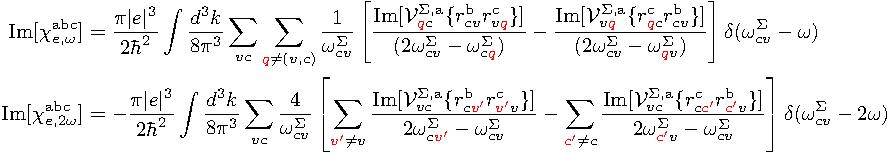
\includegraphics[scale=0.70]{chis_inter_red}
% \end{figure}
% \end{block}
% \begin{alertblock}{Intraband Contribution {\tiny $\langle n\mathbf{k}\vert
% \mathbf{r}_{i} |m\mathbf{k}'\rangle = \delta_{nm}
% \left[\delta(\mathbf{k} - \mathbf{k}')\boldsymbol{\xi}_{nn}(\mathbf{k}) +
% i\nabla_{\mathbf{k}}\delta(\mathbf{k} - \mathbf{k}')\right]$}}
% \begin{figure}
% \centering
% 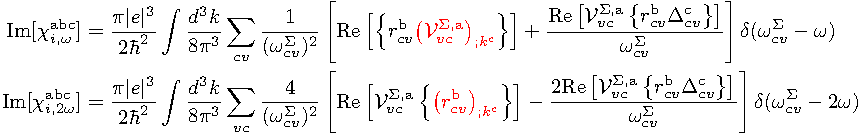
\includegraphics[scale=0.70]{chis_intra_red}
% \end{figure}
% \end{alertblock}
% \end{frame}


\subsection{Software}

\begin{frame}
Medusa runs on free and open source software:
\begin{itemize}
\item CentOS 6.7 GNU/Linux
\item Intel MPI \& OpenMP
\item Intel MKL
\item Intel FORTRAN \& C
\item Bash, Perl, Python
\end{itemize}
\begin{block}{TINIBA}
Combines Bash, Perl, Fortran, and ABINIT for calculating:
\begin{itemize}
\item Optical response of semiconductors
\item Optical response of nanomaterials
\item Spin injection in materials
\item Nonlinear optical response for surfaces and interfaces
\end{itemize}
\end{block}
\end{frame}

\begin{frame}
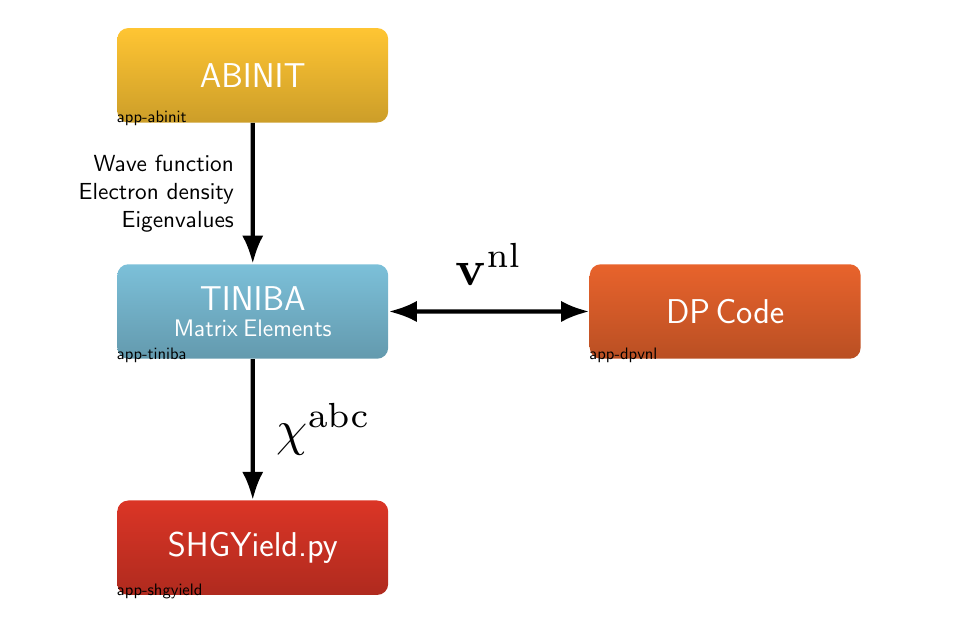
\begin{tikzpicture}[font=\sffamily,scale=0.6, every node/.style={transform shape}]
% blocks
\node [block,top color=yellow,bottom color=yellow!80!black,hyperlink node=app-abinit] at (0,10) (ABI) {\huge ABINIT};
\node [block,top color=blue,bottom color=blue!80!black,hyperlink node=app-tiniba] at (0,5) (TIN) {\huge{TINIBA}\\[4pt]\Large{Matrix Elements}};
\node [block,top color=orange,bottom color=orange!80!black,hyperlink node=app-dpvnl] at (10,5) (DP) {\huge DP Code};
\node [block,top color=red,bottom color=red!80!black,hyperlink node=app-shgyield] at (0,0) (yield) {\huge SHGYield.py};
% arrows
\draw [-Latex,ultra thick] (ABI) -- (TIN);
\draw [Latex-Latex,ultra thick] (DP) -- (TIN);
\draw [-Latex,ultra thick] (TIN) -- (yield);
% text
\node [text width=3cm,align=right,scale=1.4] at (-2.5,7.5) {Wave function\\ Electron density\\ Eigenvalues};
\node [scale=3] at (1.5,2.5) {$\chi^{\mathrm{abc}}$};
\node [scale=3] at (5,6) {$\mathbf{v}^{\mathrm{nl}}$};
\end{tikzpicture}
\end{frame}

% \begin{frame}
% \begin{block}{ABINIT\footnote{X. Gonze et al. 
% \emph{Computational Materials Science}, 25:478--492, 2002} 
% \footnote{X. Gonze et al. \emph{Z. Kristallogr.}, 220:558--562, 2005} 
% \footnote{X. Gonze et al. 
% \emph{Computer Physics Communications}, 180(12):2582, 2009}}
% First-principle study of crystals, molecules, nanostructures using density
% functional theory, many-body perturbation theory, plane waves, and
% pseudopotentials to calculate
% \begin{itemize}
% \item Electronic structure
% \item Total energy
% \item Dielectric properties, and many, many more
% \end{itemize}
% \end{block}
% \end{frame}

% \begin{frame}
% \begin{block}{DP/EXC%
% \footnote{Olevano, V. and Reining, L. and Sottile, F.,
% http://dp-code.org, http://etsf.polytechnique.fr/exc/}}

% Linear response time-dependent density-functional theory (LR-TDDFT) code in
% frequency reciprocal ($\mathbf{k}-\omega$) space on a plane waves (PW) basis
% set, for dielectric and optical Spectroscopy.
% \begin{itemize}
% \item Optical absorption
% \item Reflectivity
% \item Refraction Indices
% \item EELS
% \end{itemize}
% \end{block}
% In our case, we use DP for calculating the contribution from
% $\mathbf{v}^\mathrm{nl}$.
% \end{frame}


%%%%%%%%%%%%%%%%%%%%%%%%%%%%%%%%%%%%%%%%%%%%%%%%%%%%%%%%%%%%%%%%%%%%%%%%%%%%%%%%

\subsection{Results for \texorpdfstring{$\boldsymbol{\chi}$}{X}:
\texorpdfstring{Si(001)(2$\times$1)}{Si(001)(2x1)}}

\begin{frame}
\frametitle{The Si(001)(2$\times$1) Slab}
\begin{figure}
\centering
\includegraphics[height=0.76\textheight]{struc-Si2x1-rot}
\vspace*{-0.4cm}
\caption{Convergence is achieved with 32 layers of Si.}
\end{figure}
\end{frame}

\begin{frame}
\frametitle{Half-slab vs. Full-slab}
\begin{figure}
\centering
\includegraphics[width=0.9\textwidth]{fig-Si2x1-hsvsfs}
\caption{More layers would produce even better results.}
\end{figure}
\end{frame}

\begin{frame}
\frametitle{Top vs. Bottom Surfaces}
\begin{figure}
\centering
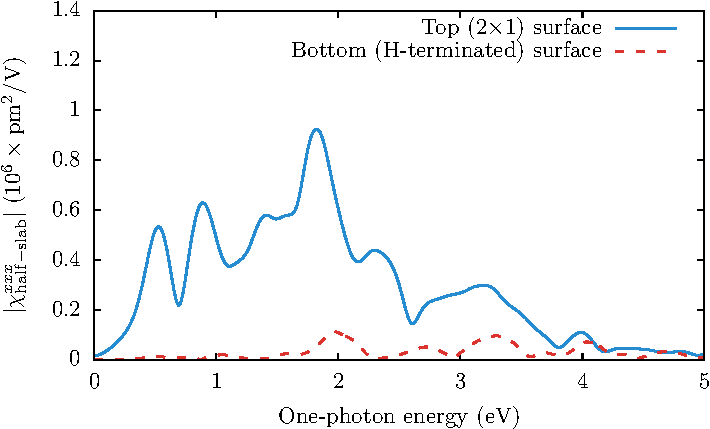
\includegraphics[width=0.9\textwidth]{fig-Si2x1-topvbottom}
\caption{Improved with more layers and more precise division of slab.}
\end{figure}
\end{frame}

\begin{frame}
\frametitle{Three Values of the Scissors Correction}
\begin{figure}
\centering
\includegraphics[width=0.9\textwidth]{fig-Si2x1-scissors}
\caption{The 2$\times$1 reconstructed surface has surface states, so the
spectrum shifts non-rigidly.}
\end{figure}
\end{frame}

\begin{frame}
\frametitle{With and Without \texorpdfstring{$\mathbf{v}^{\mathrm{nl}}$}{vnl}}
\begin{figure}
\centering
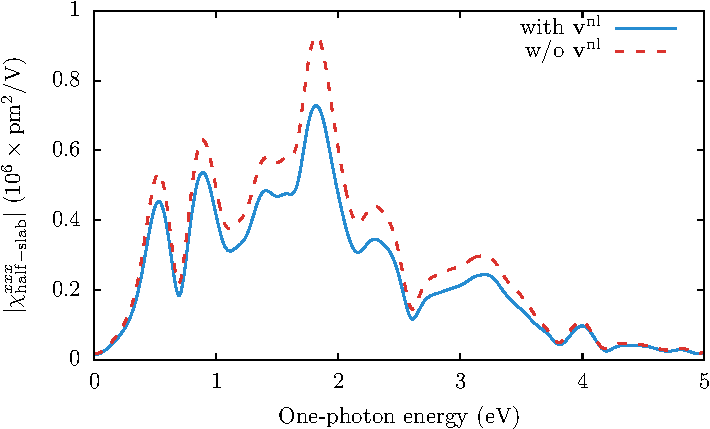
\includegraphics[width=0.9\textwidth]{fig-Si2x1-vnl}
\caption{The effect of the nonlocal part of the pseudopotentials maintains the
same line-shape but reduces the value by 15-20\% on average.}
\end{figure}
\end{frame}


%%%%%%%%%%%%%%%%%%%%%%%%%%%%%%%%%%%%%%%%%%%%%%%%%%%%%%%%%%%%%%%%%%%%%%%%%%%%%%%%

\subsection{Results for \texorpdfstring{$\boldsymbol{\chi}$}{X}:
\texorpdfstring{Si(111)(1$\times$1):H}{Si(111)(1x1):H}}

\begin{frame}
\frametitle{The Si(111)(1$\times$1):H surface}
\begin{figure}
\centering
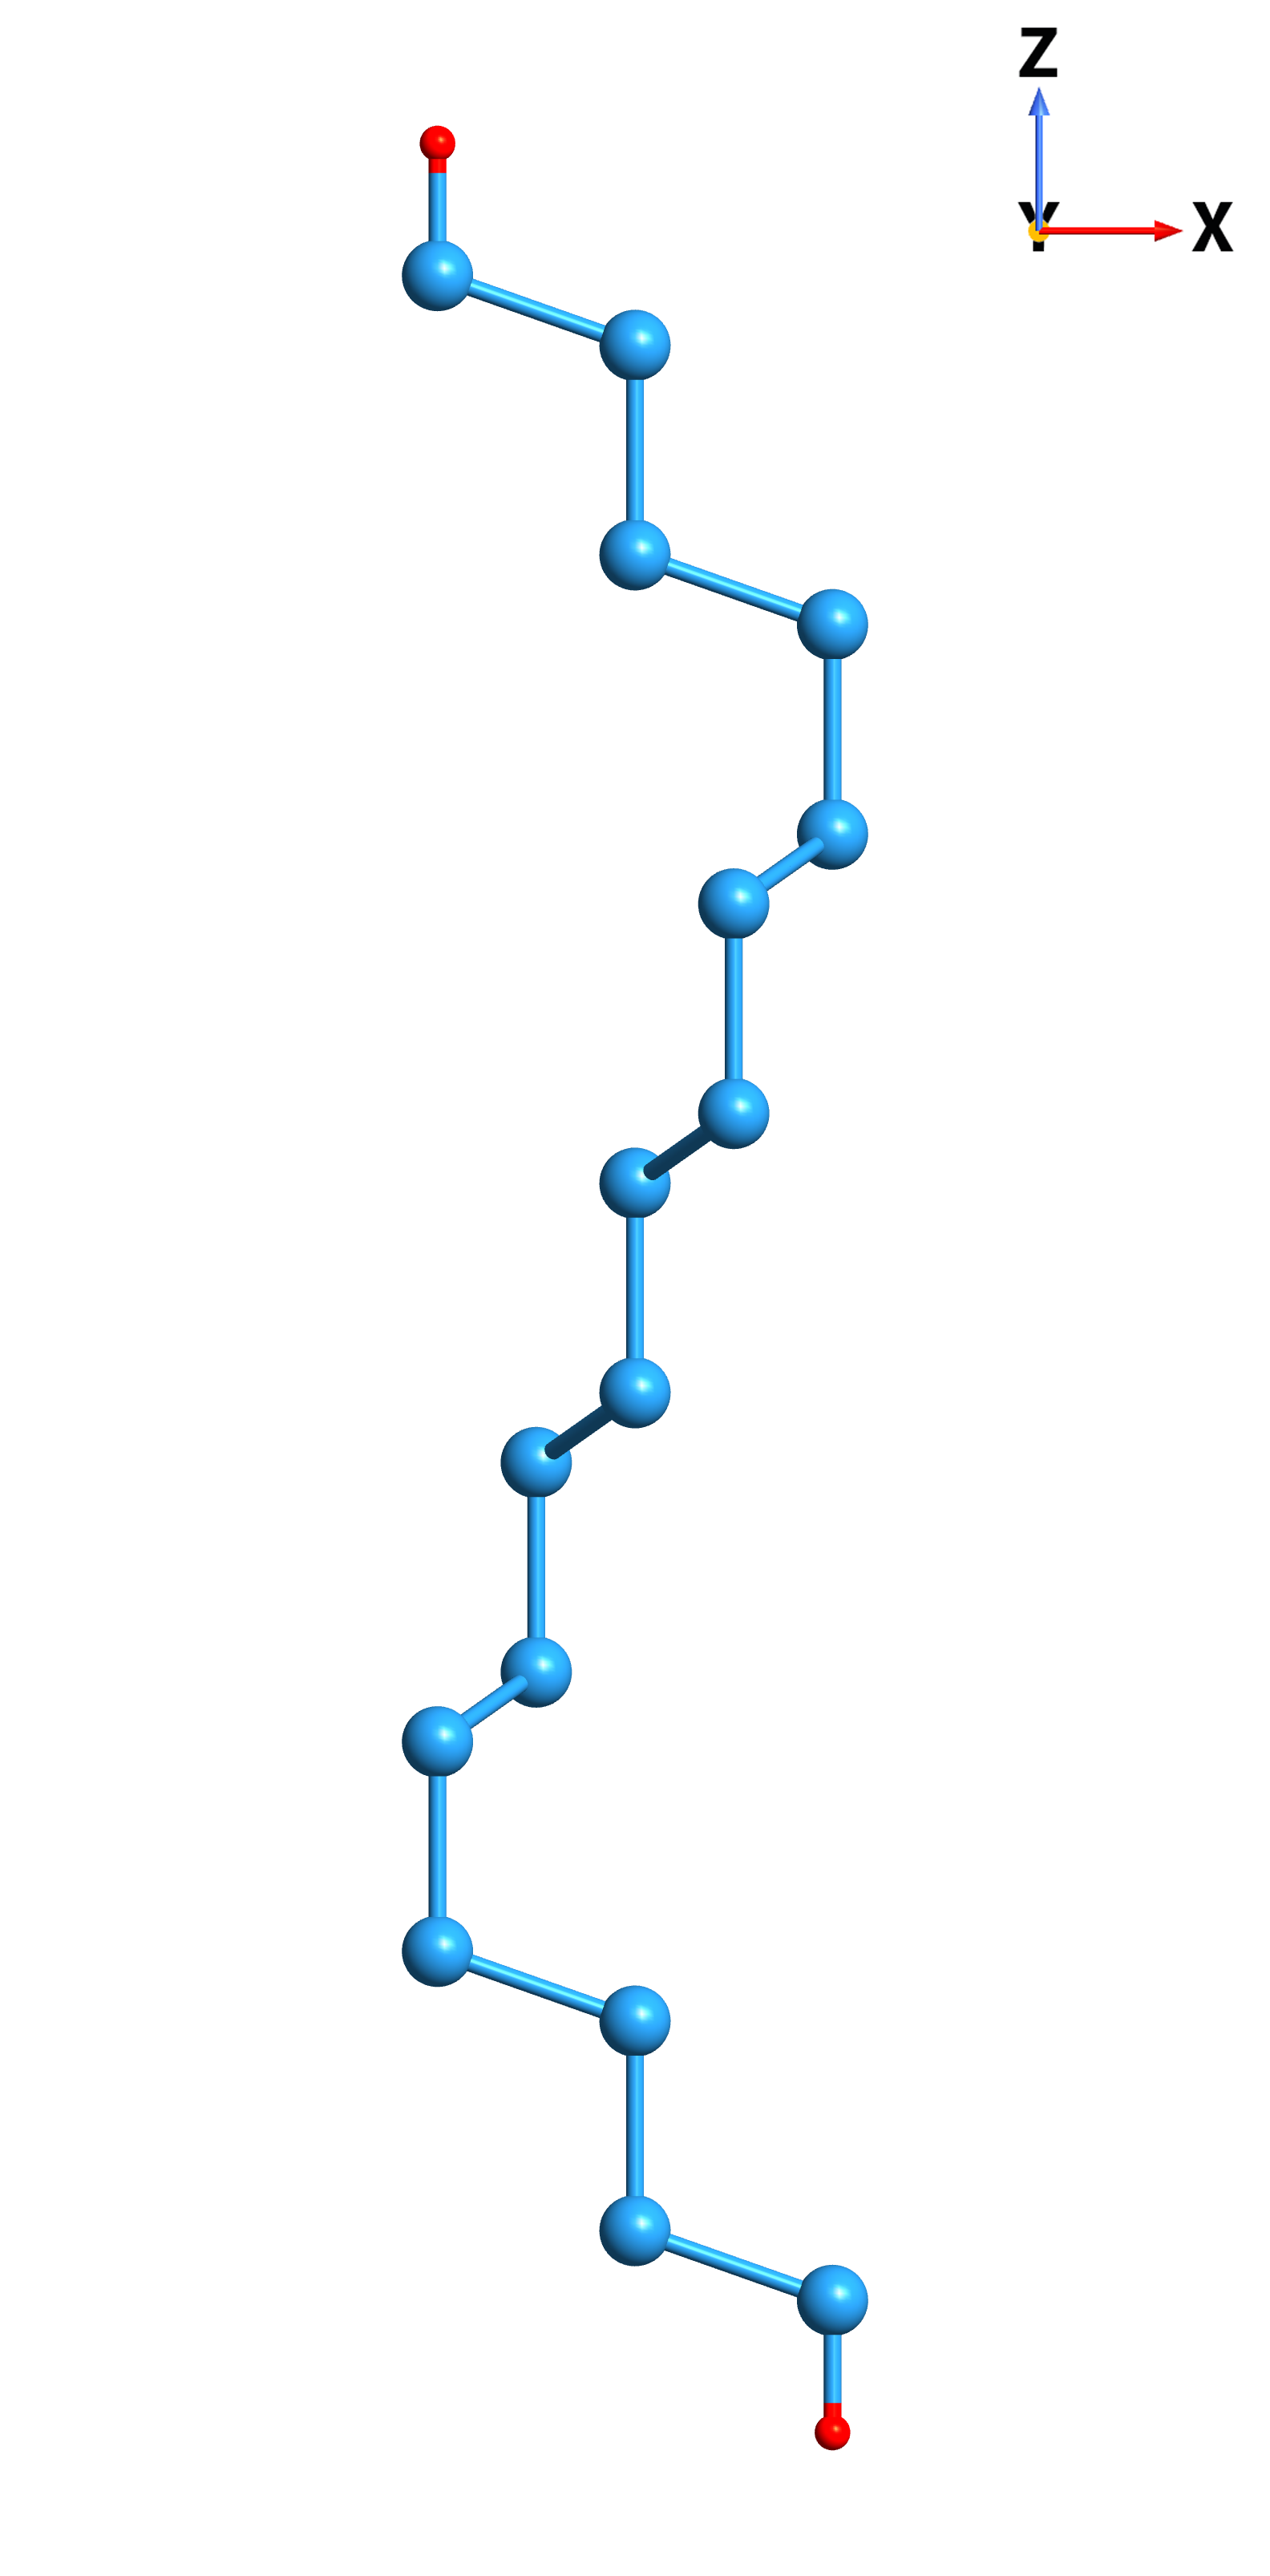
\includegraphics[height=0.7\textheight]{struc-Si1x1-front}
\caption{Si(111)(1$\times$1):H}
\end{figure}
\end{frame}

\begin{frame}
\frametitle{$\boldsymbol{\chi}$ for the Si(111)(1$\times$1):H surface%
\footnote{Experimental data from \emph{H\"ofer et al.}, 
Appl. Phys. A 63, 533 (1996)}}
\vspace{-0.5cm}
\begin{figure}
\centering
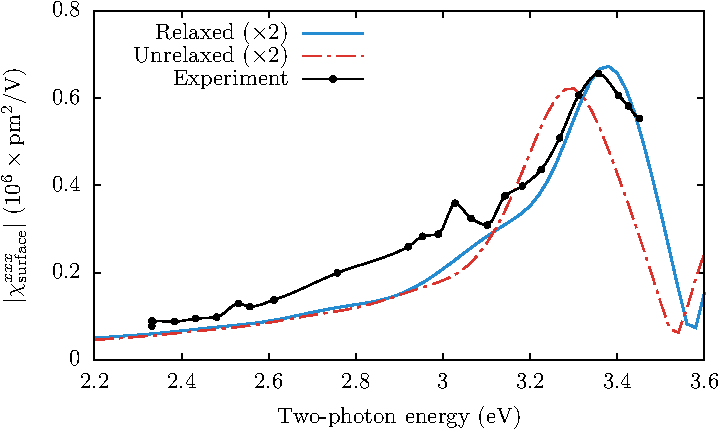
\includegraphics[width=0.65\textwidth]{fig-Si1x1-Hofer_Xxxx}
\end{figure}
\vspace{-0.5cm}
\begin{block}{Relaxing the Structure}
\begin{enumerate}
\item Worth the time and effort
\item Experimental data taken at low temperature
\end{enumerate}
\end{block}
\end{frame}


%%%%%%%%%%%%%%%%%%%%%%%%%%%%%%%%%%%%%%%%%%%%%%%%%%%%%%%%%%%%%%%%%%%%%%%%%%%%%%%%
%%%%%%%%%%%%%%%%%%%%%%%%%%%%%%%%%%%%%%%%%%%%%%%%%%%%%%%%%%%%%%%%%%%%%%%%%%%%%%%%

\section{The SSHG Yield}


%%%%%%%%%%%%%%%%%%%%%%%%%%%%%%%%%%%%%%%%%%%%%%%%%%%%%%%%%%%%%%%%%%%%%%%%%%%%%%%%

\subsection{Deriving \texorpdfstring{$\mathcal{R}$}{R}}

\begin{frame}
\frametitle{The Three Layer Model}
\begin{figure}
\centering
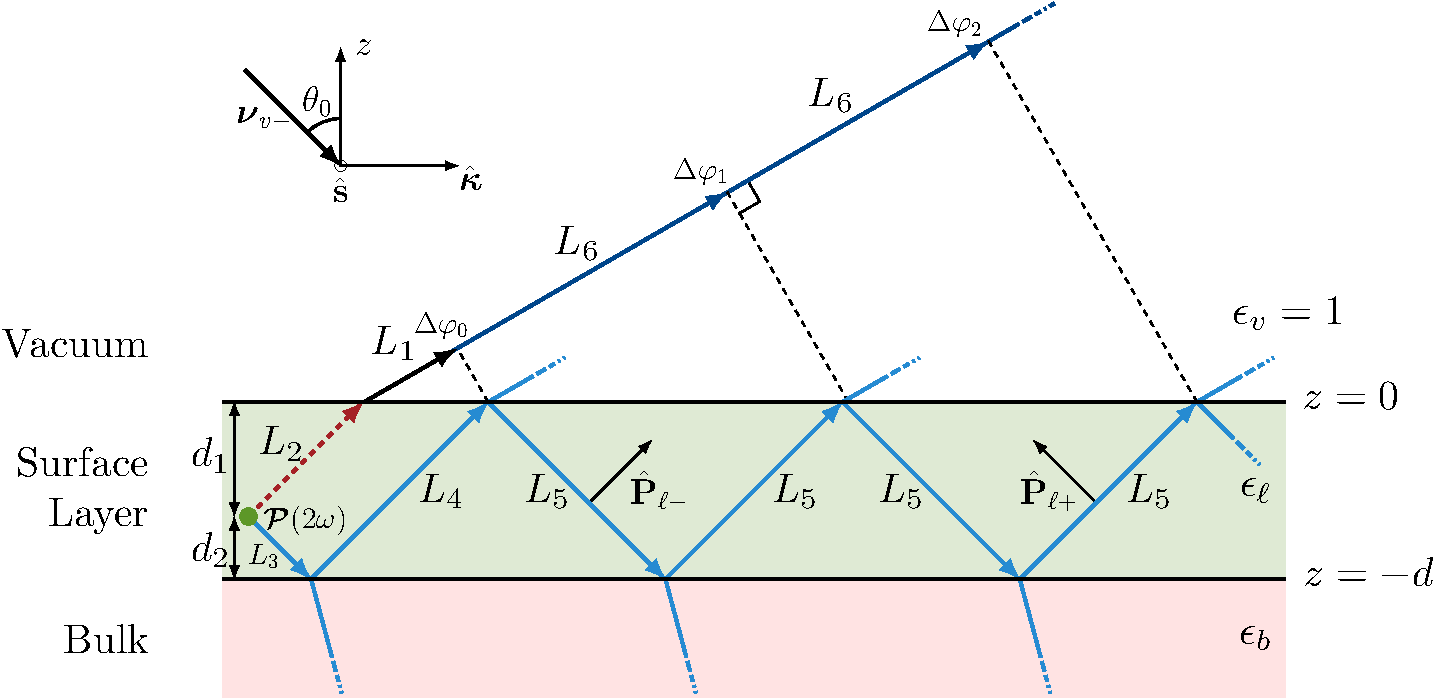
\includegraphics[width=\textwidth]{diag-3layer_MR_2w}
\caption{The nonlinear process occurs in a thin layer ($\ell$) just below the
surface, between the vacuum region ($v$) and the material bulk ($b$)}
\end{figure}
\end{frame}

\begin{frame}
\frametitle{Explicit Expressions for $\mathcal{R}$%
\footnote{\emph{Anderson, et al.}, Phys. Rev. B 93, 235304 (2016)}
\footnote{\emph{Anderson, et al.}, Phys. Rev. B, submitted}
}
The SSHG yield is
\begin{equation*}
\mathcal{R}_{\mathrm{iF}}(2\omega) =
\frac{\omega^{2}}{2\epsilon_{0}c^3\cos^{2}\theta_{0}}
\left\vert\frac{1}{n_{\ell}}\Upsilon_{\mathrm{iF}}\right\vert^{2}
\quad\left[\frac{\mathrm{m}^{2}}{\mathrm{W}}\right]
\end{equation*}
for each combination of polarizations of incoming and outgoing fields
($\mathrm{iF} = pP, pS, sP,$ and $sS$). We have that
\begin{equation*}\label{eq:mc25}
\Upsilon_{\mathrm{iF}} = \Gamma_{\mathrm{iF}}\,r_{\mathrm{iF}},
\end{equation*}
where,
$$
\begin{array}{ l l }
\Gamma_{pP} =
\frac{T^{v\ell}_{p}}{N_{\ell}}
\left(\frac{t^{v\ell}_{p}}{n_{\ell}}\right)^{2},
&
\Gamma_{sP}=
\frac{T^{v\ell}_{p}}{N_{\ell}}
\left(t^{v\ell}_{s}r^{M+}_{s}\right)^{2},\quad\\
\Gamma_{pS} =
T_{s}^{v\ell}R^{M+}_{s}
\left(\frac{t^{v\ell}_{p}}{n_{\ell}}\right)^{2},\quad
&
\Gamma_{sS} = 
T_{s}^{v\ell}R^{M+}_{s}\left(t^{v\ell}_{s}r^{M+}_{s}\right)^{2},
\end{array}
$$
\end{frame}

\begin{frame}
\frametitle{Explicit Expressions for $\mathcal{R}$}
In particular, for the (111) surface we have
\begin{align*}
r^{(111)}_{pP} &= 
R^{M+}_{p}\sin\theta_{0}
\Big[
  \left(r^{M+}_{p}\right)^{2}\sin^{2}\theta_{0}\chi^{zzz}
+ \left(r^{M-}_{p}\right)^{2}w^{2}_{\ell}\chi^{zxx}
\Big]\\
&- R^{M-}_{p}w_{\ell}W_{\ell}
\Big[
  2r^{M+}_{p}r^{M-}_{p}\sin\theta_{0}\chi^{xxz}
+ \left(r^{M-}_{p}\right)^{2}w_{\ell}\chi^{xxx}\cos3\phi
\Big],\\\\
r^{(111)}_{sP} &= 
R^{M+}_{p}\sin\theta_{0}\chi^{zxx} +
R^{M-}_{p}W_{\ell}\chi^{xxx}\cos3\phi,\\\\
r^{(111)}_{pS} &= - \left(r^{M-}_{p}\right)^{2}w^{2}_{\ell}\chi^{xxx}\sin3\phi,\\\\
r^{(111)}_{sS} &= \chi^{xxx}\sin3\phi.
\end{align*}
\end{frame}

% \begin{frame}
% \frametitle{About the Code}
% \begin{block}{SHGYield.py}
% A python script designed to calculate the nonlinear reflection coefficient for
% semiconductor surfaces. It works in conjunction with the matrix elements
% calculated with ABINIT, an open source \emph{ab initio} software, and TINIBA,
% our in-house optical calculation software.
% \begin{itemize}
% \item Reads necessary data from input file
% \item Works for any angles
% \item Allows selection of other models besides three-layer
% \item Can include or neglect effects of multiple reflections
% \end{itemize}
% \end{block}
% Get it at: https://github.com/roguephysicist/SHGYield
% \end{frame}


%%%%%%%%%%%%%%%%%%%%%%%%%%%%%%%%%%%%%%%%%%%%%%%%%%%%%%%%%%%%%%%%%%%%%%%%%%%%%%%%

\subsection{Results for \texorpdfstring{$\mathcal{R}$}{R}: 
Si(111)(1\texorpdfstring{$\times$}{x}1):H}

\begin{frame}
\frametitle{Si(111)(1\texorpdfstring{$\times$}{x}1):H -- Outgoing
\texorpdfstring{$P$}{P} polarization}
\begin{columns}
\column{0.55\textwidth}
\begin{figure}
\centering
\includegraphics[width=\textwidth]{3D-Si1x1-RpP}
\caption{$\mathcal{R}_{pP}$ with $\phi=45$}
\end{figure}
\column{0.55\textwidth}
\begin{figure}
\centering
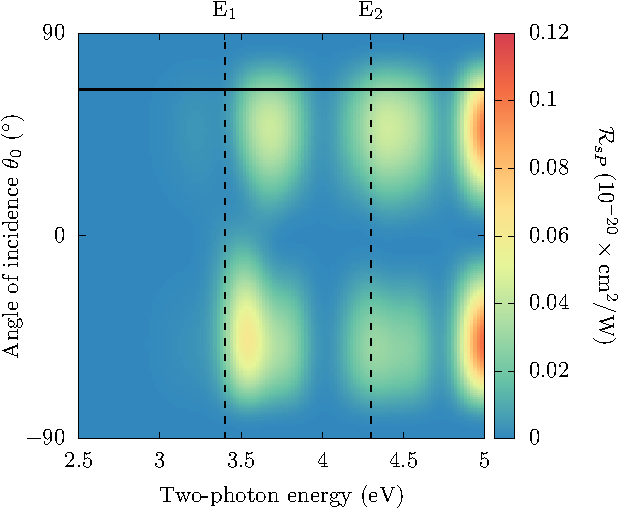
\includegraphics[width=\textwidth]{3D-Si1x1-RsP}
\caption{$\mathcal{R}_{sP}$ with $\phi=45$}
\end{figure}
\end{columns}
\end{frame}

\begin{frame}
\frametitle{Si(111)(1\texorpdfstring{$\times$}{x}1):H -- Outgoing
\texorpdfstring{$S$}{S} polarization}
\begin{columns}
\column{0.55\textwidth}
\begin{figure}
\centering
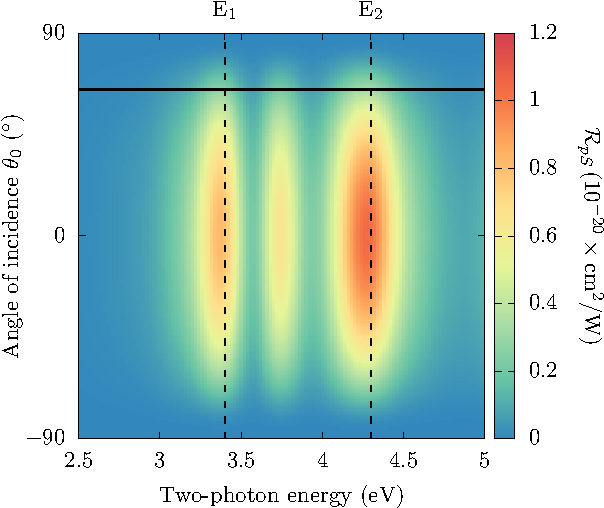
\includegraphics[width=\textwidth]{3D-Si1x1-RpS}
\caption{$\mathcal{R}_{pS}$ with $\phi=45$}
\end{figure}
\column{0.55\textwidth}
\begin{figure}
\centering
\includegraphics[width=\textwidth]{3D-Si1x1-RsS}
\caption{$\mathcal{R}_{sS}$ with $\phi=45$}
\end{figure}
\end{columns}
\end{frame}

\begin{frame}
\frametitle{Si(111)(1\texorpdfstring{$\times$}{x}1):H -- 
\texorpdfstring{$\mathcal{R}_{pP}$}{RpP} at
\texorpdfstring{$E_{1} = 3.4$}{E1 = 3.4} eV}
\begin{columns}
\column{0.5\textwidth}
\begin{figure}
\centering
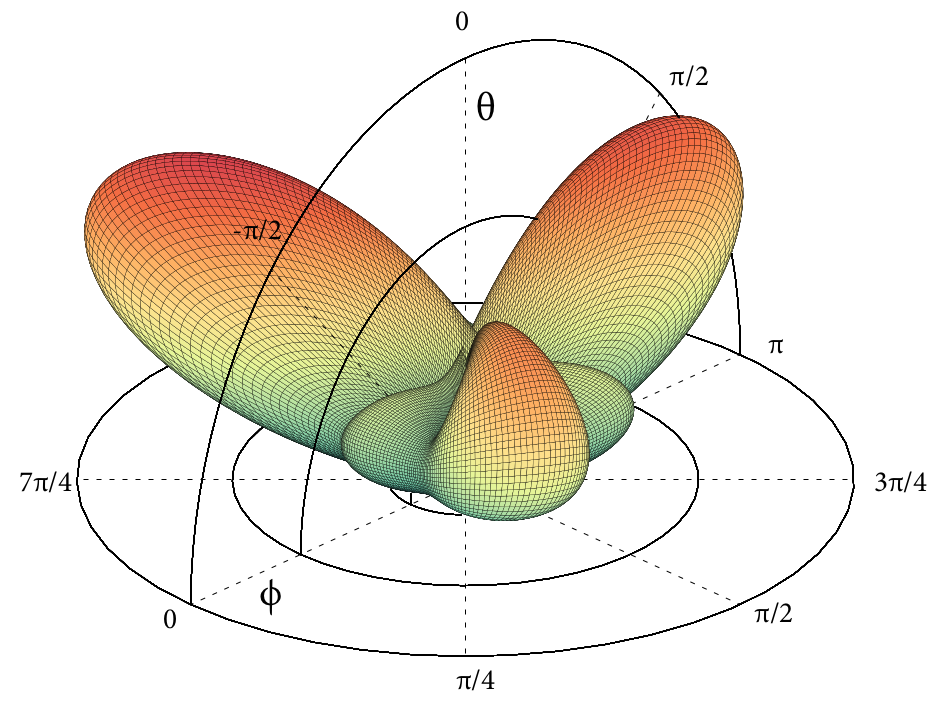
\includegraphics[height=0.6\textheight]{3Dside01}
\end{figure}
\column{0.5\textwidth}
\begin{figure}
\centering
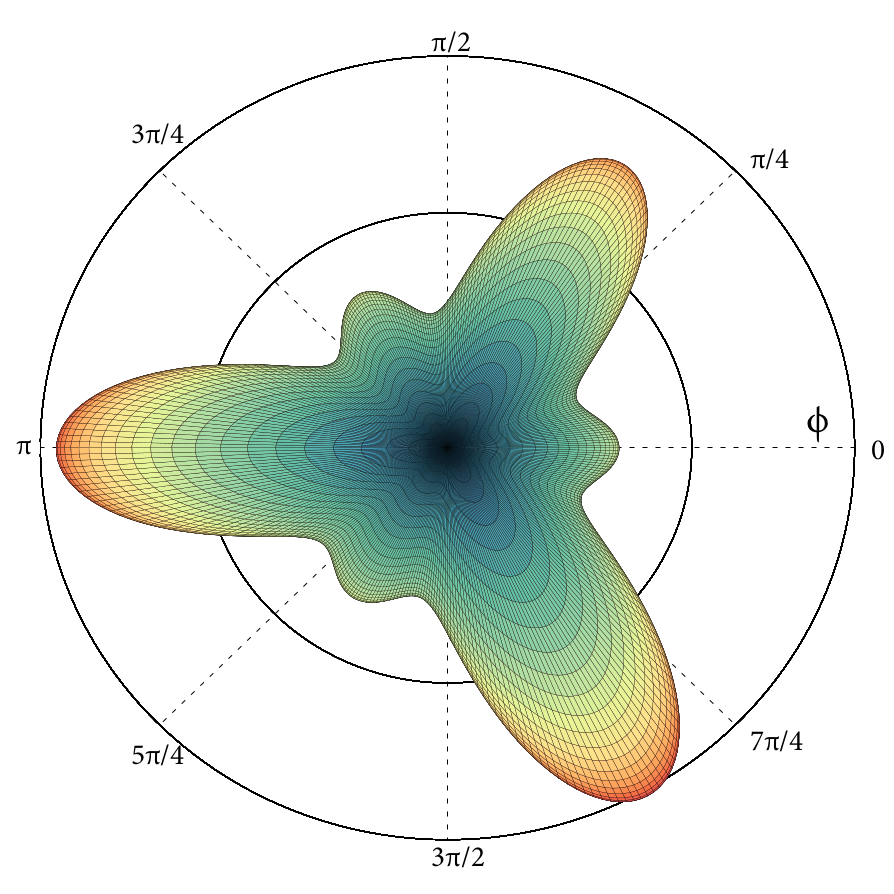
\includegraphics[height=0.6\textheight]{3Dtop}
\end{figure}
\end{columns}
\end{frame}

\begin{frame}
% \frametitle{Si(111)(1\texorpdfstring{$\times$}{x}1):H -- $\mathcal{R}_{pP}$}
\begin{figure}
\centering
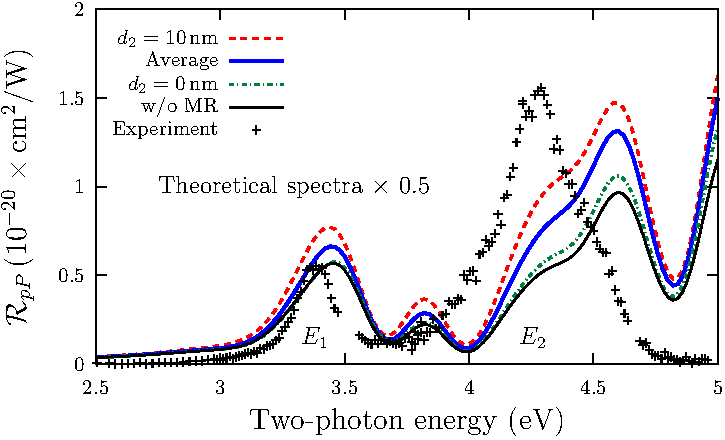
\includegraphics[width=\textwidth]{fig-Si1x1-MRdepth}
\caption{$\mathcal{R}_{pP}$ for $\theta=65$ and $\phi=45$ at room temperature%
\footnote{Experimental data from \emph{Mejia et al.}, Phys. Rev. B 66, 195329 (2002)}}
\end{figure}
\end{frame}

\begin{frame}
\frametitle{The Three Layer Model}
\begin{figure}
\centering
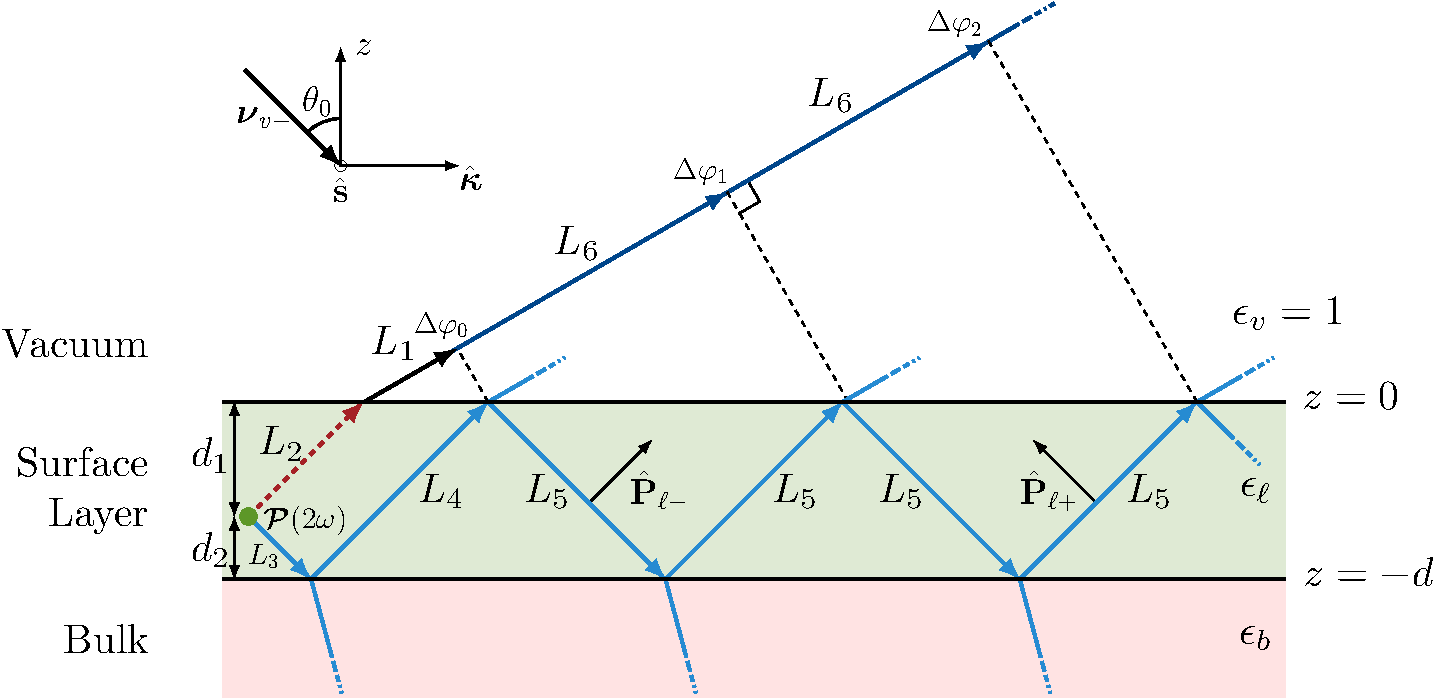
\includegraphics[width=\textwidth]{diag-3layer_MR_2w}
\caption{The nonlinear process occurs in a thin layer ($\ell$) just below the
surface, between the vacuum region ($v$) and the material bulk ($b$)}
\end{figure}
\end{frame}

\begin{frame}
\frametitle{Other models}
\begin{figure}
\centering
\includegraphics[width=\textwidth]{fig-Si1x1-Mejia_RpP}
\end{figure}
\end{frame}

\begin{frame}
\frametitle{Other models}
\begin{figure}
\centering
\includegraphics[width=\textwidth]{fig-Si1x1-Mejia_RpP_models}
\end{figure}
\end{frame}

\begin{frame}
% \frametitle{Si(111)(1\texorpdfstring{$\times$}{x}1):H -- $\mathcal{R}_{pS}$}
\begin{figure}
\centering
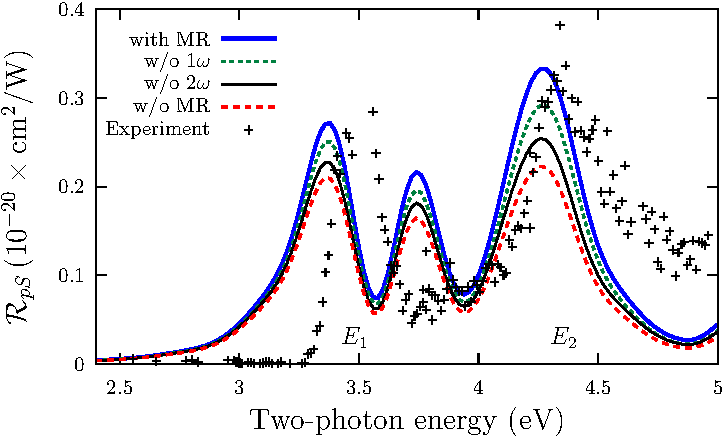
\includegraphics[width=\textwidth]{fig-Si1x1-Mejia_RpS}
\caption{$\mathcal{R}_{pS}$ for $\theta=65$ and $\phi=45$ at room temperature%
\footnote{Experimental data from \emph{Mejia et al.}, Phys. Rev. B 66, 195329 (2002)}}
\end{figure}
\end{frame}

\begin{frame}
% \frametitle{Si(111)(1\texorpdfstring{$\times$}{x}1):H -- $\mathcal{R}_{sP}$}
\begin{figure}
\centering
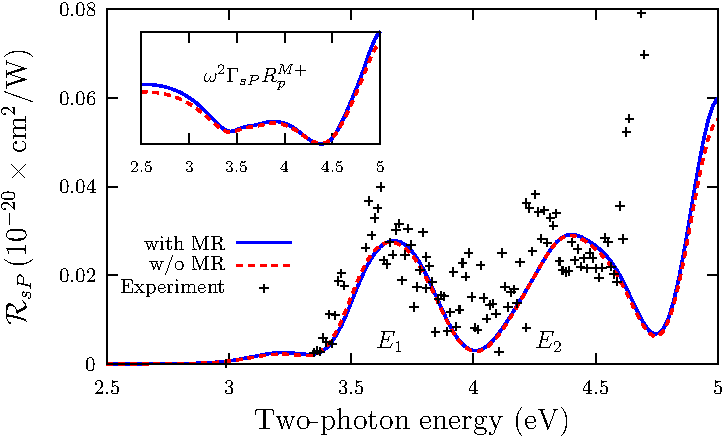
\includegraphics[width=\textwidth]{fig-Si1x1-Mejia_RsP}
\caption{$\mathcal{R}_{sP}$ for $\theta=65$ and $\phi=45$ at room temperature%
\footnote{Experimental data from \emph{Mejia et al.}, Phys. Rev. B 66, 195329 (2002)}}
\end{figure}
\end{frame}

\begin{frame}
\frametitle{\texorpdfstring{$\mathcal{R}_{pP}$}{RpP} -- Old vs. New}
\begin{columns}
\column{0.55\textwidth}
\begin{figure}
\centering
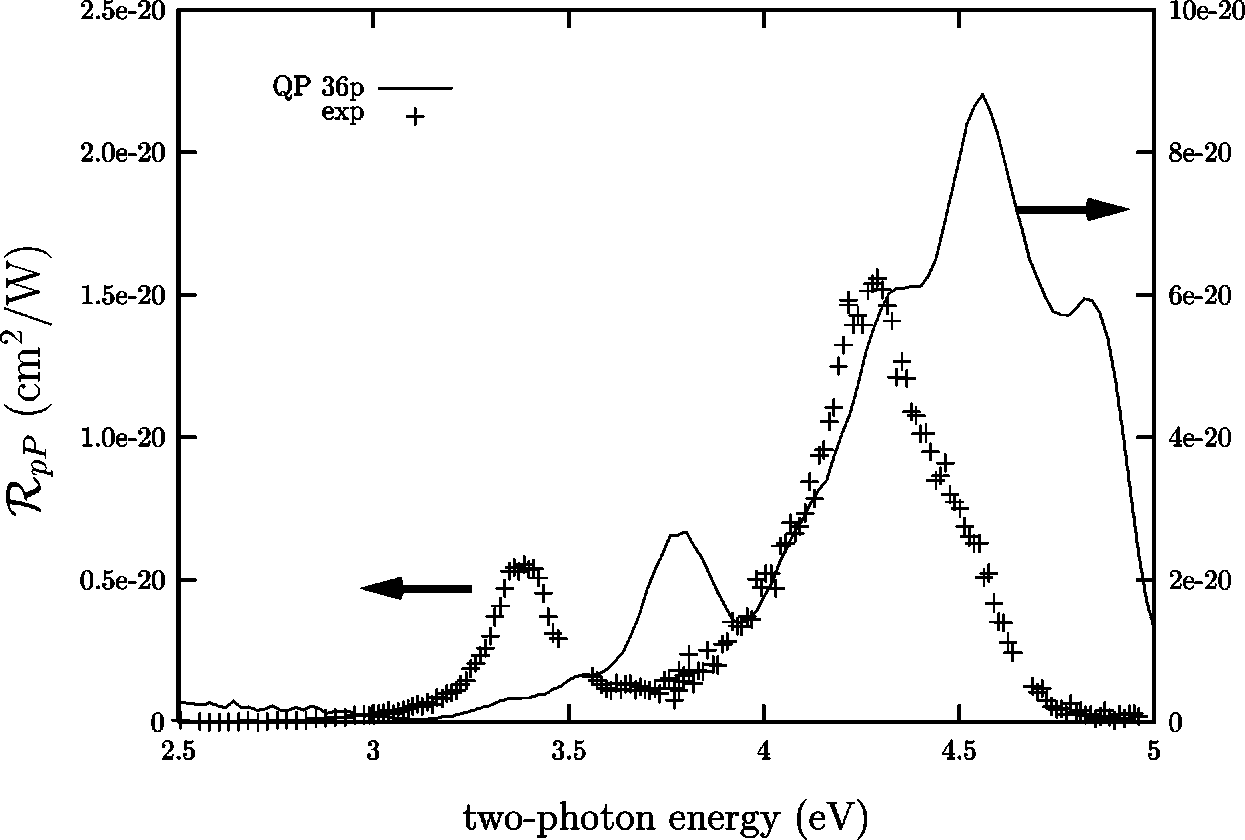
\includegraphics[width=\textwidth]{mejia-000}
\caption{From \emph{Mejia et al.}}
\end{figure}
\column{0.55\textwidth}
\begin{figure}
\centering
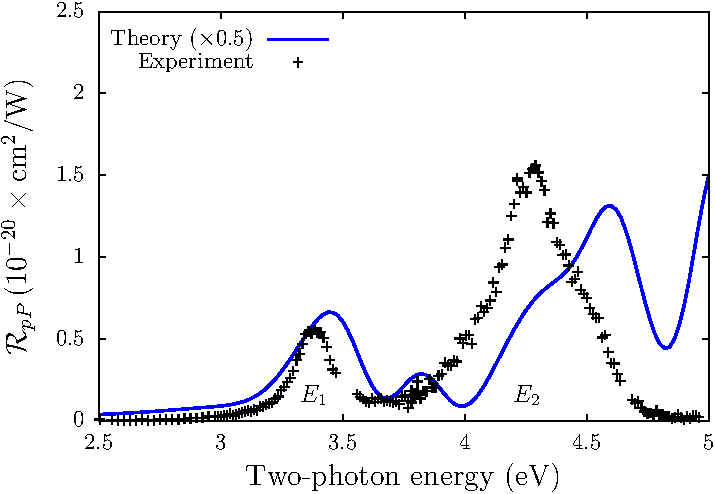
\includegraphics[width=\textwidth]{fig-rpp}
\caption{This work.}
\end{figure}
\end{columns}
\end{frame}

\begin{frame}
\frametitle{\texorpdfstring{$\mathcal{R}_{pS}$}{RpS} -- Old vs. New}
\begin{columns}
\column{0.55\textwidth}
\begin{figure}
\centering
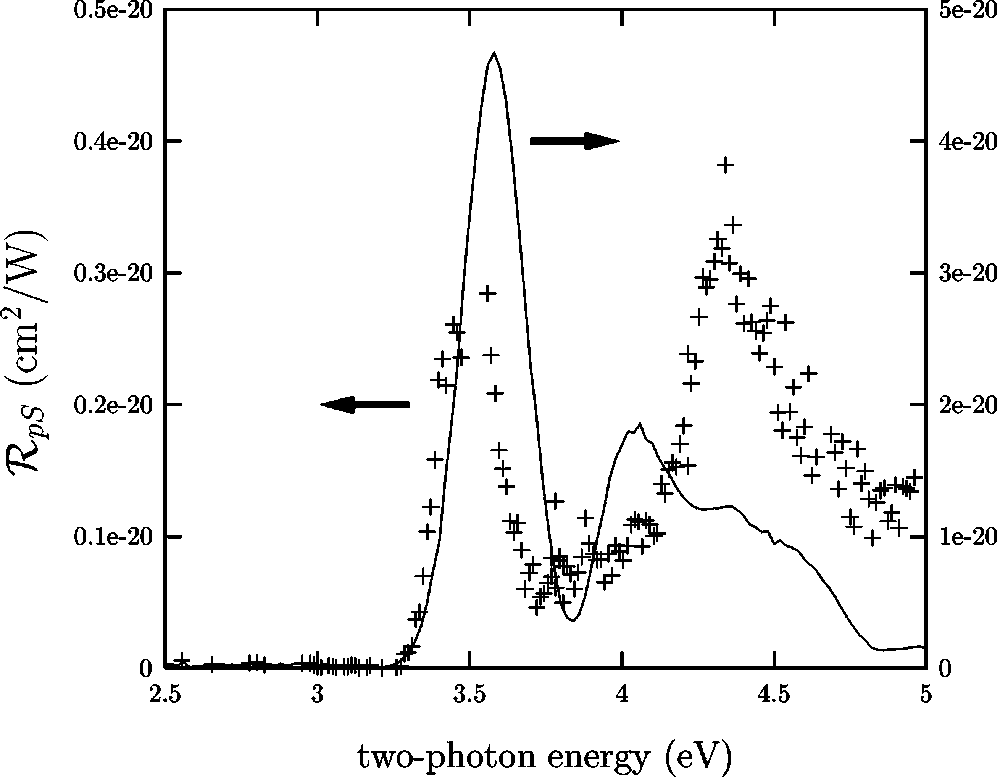
\includegraphics[width=\textwidth]{mejia-001}
\caption{From \emph{Mejia et al.}}
\end{figure}
\column{0.55\textwidth}
\begin{figure}
\centering
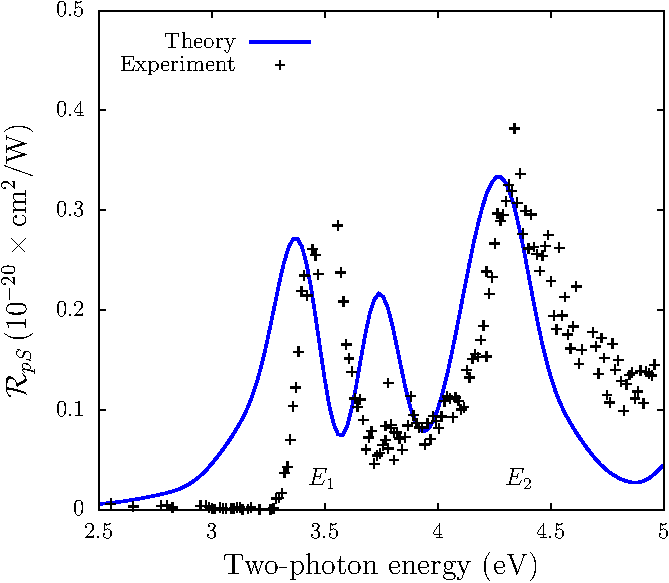
\includegraphics[width=0.9\textwidth]{fig-rps}
\caption{This work.}
\end{figure}
\end{columns}
\end{frame}

\begin{frame}
\frametitle{Summary}
\begin{itemize}
\item Intensity is very close to experiment with unambiguous units. No more arbitrary units!
\item Peak position is also quite close, temperature effects are clear.
\item Multiple reflections enhances peak proportions and intensity according to experiment.
\item We can now have \emph{quantitative} and predictive results for any surface!
\end{itemize}
\end{frame}


%%%%%%%%%%%%%%%%%%%%%%%%%%%%%%%%%%%%%%%%%%%%%%%%%%%%%%%%%%%%%%%%%%%%%%%%%%%%%%%%
%%%%%%%%%%%%%%%%%%%%%%%%%%%%%%%%%%%%%%%%%%%%%%%%%%%%%%%%%%%%%%%%%%%%%%%%%%%%%%%%

\section{Conclusions}


%%%%%%%%%%%%%%%%%%%%%%%%%%%%%%%%%%%%%%%%%%%%%%%%%%%%%%%%%%%%%%%%%%%%%%%%%%%%%%%%

\subsection{Methods}

\begin{frame}
\frametitle{What's Next?}
\centering
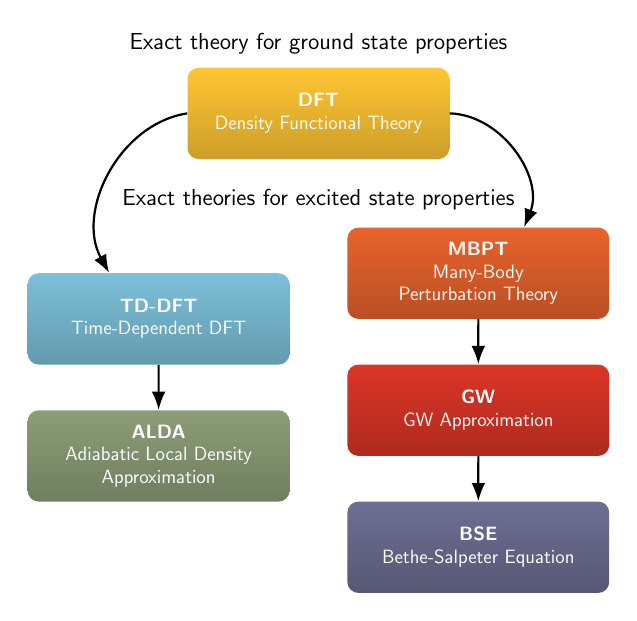
\begin{tikzpicture}[font=\sffamily\large,scale=0.58, every node/.style={transform shape}]
% blocks
\node [block,top color=yellow,bottom color=yellow!80!black] at (4,10) (DFT) 
       {\textbf{DFT}\\ Density Functional Theory};
\node [block,top color=blue,bottom color=blue!80!black] at (0.5,5.5) (TDDFT)
       {\textbf{TD-DFT}\\ Time-Dependent DFT};
\node [block,top color=green,bottom color=green!80!black] at (0.5,2.5) (ALDA)
       {\textbf{ALDA}\\ Adiabatic Local Density\\ Approximation};
\node [block,top color=orange,bottom color=orange!80!black] at (7.5,6.5) (MBPT)
       {\textbf{MBPT}\\ Many-Body\\ Perturbation Theory};
\node [block,top color=red,bottom color=red!80!black] at (7.5,3.5) (GW)
       {\textbf{GW}\\ GW Approximation};
\node [block,top color=purple,bottom color=purple!80!black] at (7.5,0.5) (BSE)
       {\textbf{BSE}\\ Bethe-Salpeter Equation};
% arrows
\draw [-Latex,thick] (DFT.west) to [bend right=55] (TDDFT);
\draw [-Latex,thick] (TDDFT) -- (ALDA);
\draw [-Latex,thick] (DFT.east) to [bend left=55] (MBPT);
\draw [-Latex,thick] (MBPT) -- (GW);
\draw [-Latex,thick] (GW) -- (BSE);
% text
\node [yshift=15] at (DFT.north) {\Large Exact theory for ground state properties};
\node [yshift=-25] at (DFT.south) {\Large Exact theories for excited state properties};
\end{tikzpicture}
\end{frame}

\begin{frame}
\frametitle{Where We Stand}
\centering
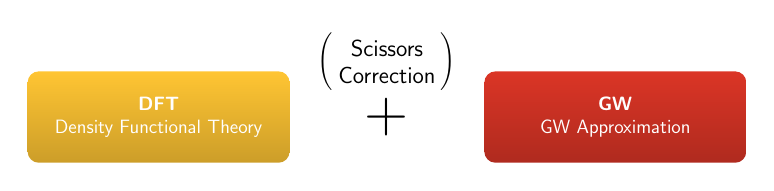
\begin{tikzpicture}[font=\sffamily\large,scale=0.58, every node/.style={transform shape}]
\node [block,top color=yellow,bottom color=yellow!80!black] at (0,0) (DFT) 
       {\textbf{DFT}\\ Density Functional Theory};
\node [scale=3] at (5,0) (plus) {$+$};
\node [block,top color=red,bottom color=red!80!black] at (10,0) (GW)
       {\textbf{GW}\\ GW Approximation};
\node [scale=1.2,yshift=10,text width=2cm,align=center] at (plus.north) (scis) {Scissors\\ Correction};
\node at (scis.west) {\Bigg(};
\node at (scis.east) {\Bigg)};
\end{tikzpicture}
\begin{columns}
\column{0.5\textwidth}
\begin{figure}
\centering
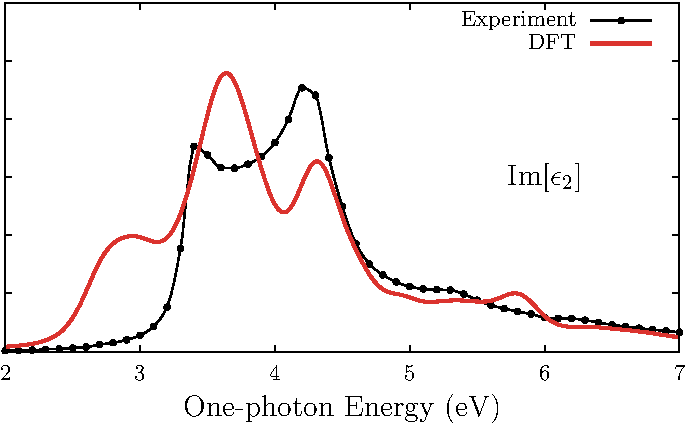
\includegraphics[width=\textwidth]{fig-mbpt01}
\end{figure}
\column{0.5\textwidth}
\begin{figure}
\centering
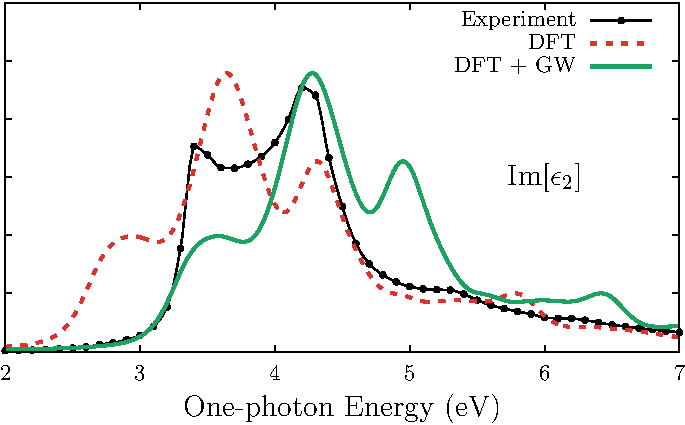
\includegraphics[width=\textwidth]{fig-mbpt02}
\end{figure}
\end{columns}
\end{frame}

\begin{frame}
\frametitle{The State of the Art}
\centering

\begin{tikzpicture}[font=\sffamily\large]
\node [block,top color=purple,bottom color=purple!80!black] at (0,0) (BSE)
       {\textbf{BSE}\\ Bethe-Salpeter Equation};
\end{tikzpicture}
\begin{figure}
\centering
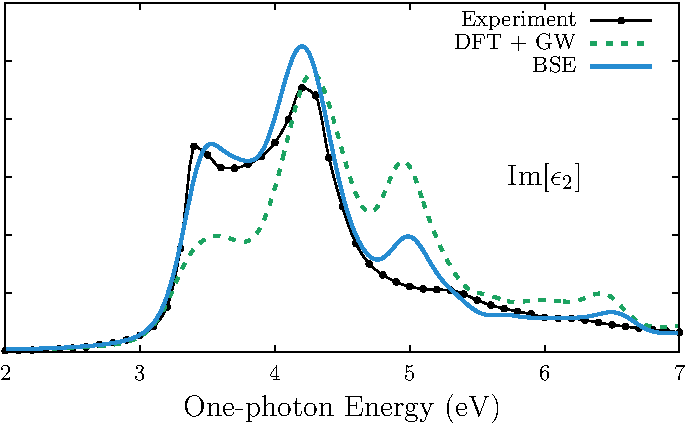
\includegraphics[height=0.55\textheight]{fig-mbpt03}
\end{figure}
\end{frame}

% \begin{frame}
% \frametitle{Fat Nodes $\rightarrow$ Up to 6 TB of RAM!}
% \vspace{-0.5cm}
% \begin{figure}
% \centering
% \includegraphics[width=1.01\textwidth]{image-fats}
% \end{figure}
% \end{frame}

%%%%%%%%%%%%%%%%%%%%%%%%%%%%%%%%%%%%%%%%%%%%%%%%%%%%%%%%%%%%%%%%%%%%%%%%%%%%%%%%

\subsection{Credits}

\begin{frame}
\frametitle{Productivity}
\begin{block}{Produced Articles}
\begin{itemize}
\small
\item \emph{Anderson, et al.}, Phys. Rev. B 93, 235304 (2016)
\item \emph{Zapata-Pe\~na, Anderson, et al.}, 
            Phys. Status Solidi B 253, 408 (2016) % COVER PAGE
\item \emph{Anderson, et al.}, Phys. Rev. B 91, 075302 (2015)
\item \emph{Anderson, et al.}, arXiv:1604.07722 [physics.optics] (2016)
\item \emph{Anderson, et al.}, Phys. Rev. B, Submitted (2016)
% \item \emph{Corzo-G\'arcia et al.}, Opt. Laser. Eng. 49, 1251 (2011)
\end{itemize}
\end{block}
\begin{block}{Academic Stays}
\begin{itemize}
\small
\item Laboratoire des Solides Irradi\'es, \'Ecole Polytechnique, France (2015)
\item Laboratoire des Solides Irradi\'es, \'Ecole Polytechnique, France (2014)
\end{itemize}
\end{block}
\end{frame}

\begin{frame}
% \frametitle{Productivity}
\begin{block}{Conferences}
\begin{itemize}
\item Psi-K 2015 (Ganador del Concurso de Posters Cient\'ificos)
\item OSI-11 2015 (Poster)
\item ENU-HPC 2012 (Submitted Talk)
\end{itemize}
\end{block}
\begin{block}{Specialized Courses}
\begin{itemize}
\item \emph{Ab-initio} calculations with the DP/EXC Codes (2016) (Imparted)
\item Control de versiones usando Git y GitHub (2013) (Imparted)
\item C\'omputo en paralelo mediante FORTRAN/C++ con MPI y OpenMP (2013)
\item C\'alculo de propiedades \'opticas de la materia con el uso de teor\'ia 
      de muchos cuerpos (2013)
\end{itemize}
\end{block}
\end{frame}

\begin{frame}
\frametitle{Acknowledgements}
\begin{itemize}
\item Benevolent leader: Dr. Bernardo Mendoza
\item Dr. Ram\'on Carriles Jaimes
\item Dr. Norberto Arzate Plata
\item Dr. Francisco Villa Villa
\item Dr. Wolf Luis Moch\'an Backal
\item Reinaldo Arturo Zapata Pe\~na
\item Val\'erie V\'eniard \& Nicolas Tancogne-Dejean
\item The CONACYT
\item The CIO for 6 great years
\item My parents, Mike \& Ana
\item All my friends
\item Dra. Liliana Villafa\~na L\'opez
\end{itemize}
\begin{center}
% \vspace{3em}
{\huge Thanks for coming!}
\end{center}
\end{frame}


\subsection{Appendix}

\begin{frame}
\hypertarget{app-abinit}{}
\frametitle{ABINIT}
\centering
\begin{figure}
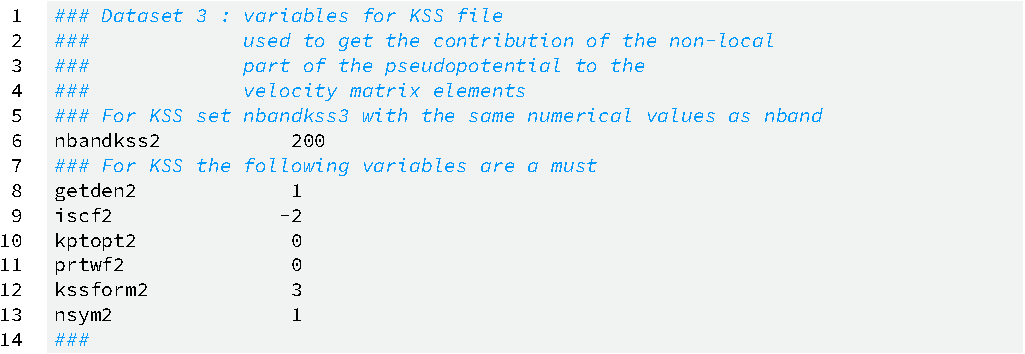
\includegraphics[width=0.9\textwidth]{code-abinit}
\end{figure}
http://www.abinit.org
\end{frame}

\begin{frame}
\hypertarget{app-tiniba}{}
\frametitle{TINIBA}
\centering
\begin{figure}
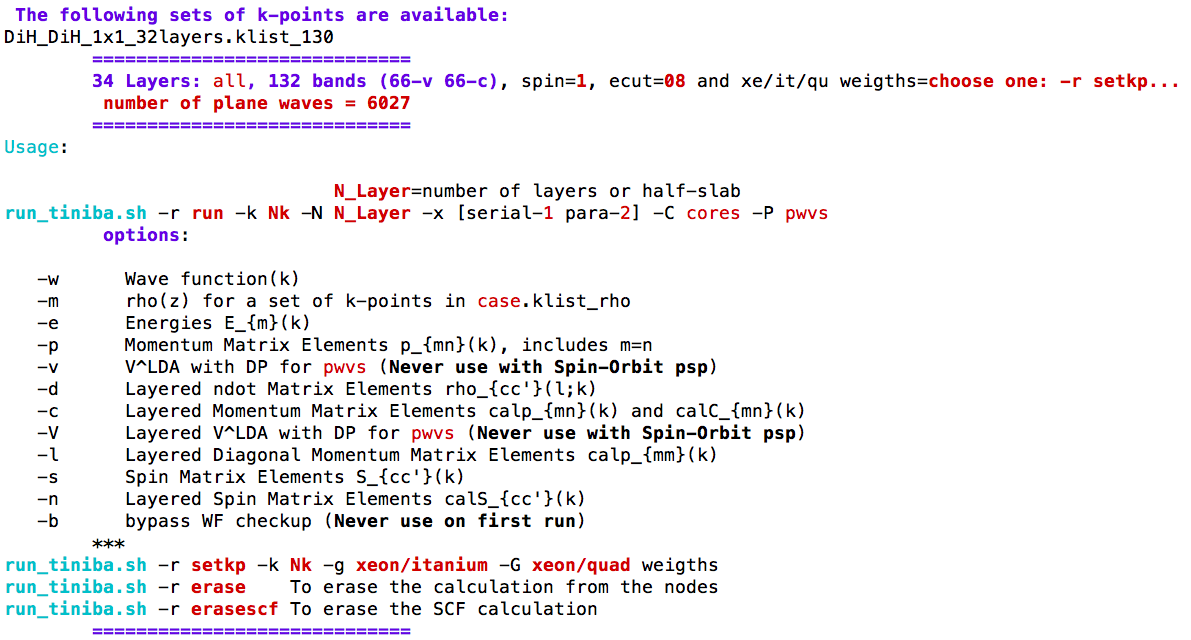
\includegraphics[width=0.9\textwidth]{image-tiniba}
\end{figure}
https://github.com/roguephysicist/tiniba-manual
\end{frame}

\begin{frame}
\hypertarget{app-dpvnl}{}
\frametitle{Contribution of the Nonlocal Part of the Pseudopotential}
\tiny
\begin{equation*}\label{vnl.14}
\begin{split}
&\boldsymbol{\mathcal{V}}^{\mathrm{nl},\ell}_{nm}(\mathbf{k}) = \frac{1}{2\hbar}
\sum_s\sum_{l=0}^{l_s}\sum_{m=-l}^{l}E_{l}\Bigg[\\
&+\Bigg(\sum_{{\mathbf{G}''}}
\nabla_{{\mathbf{G}''}}f_{lm}^s({\mathbf{G}''})
\sum_{\mathbf{G}}A^{*}_{n{\mathbf{k}}}(\mathbf{G})\delta_{\mathbf{G}_{||}{\mathbf{G}''}_{||}}
f_\ell(G_z-G''_z) \Bigg)  
\Bigg( \sum_{{\mathbf{G}'}}A_{m{\mathbf{k}}}({\mathbf{G}'})f_{lm}^{s*}({\mathbf{K}'}) \Bigg)\\%
&+ \Bigg(\sum_{{\mathbf{G}''}}
f_{lm}^s({\mathbf{G}''})\sum_{\mathbf{G}}A^{*}_{n{\mathbf{k}}}(\mathbf{G})\delta_{\mathbf{G}_{||}{\mathbf{G}''}_{||}}
f_\ell(G_z-G''_z) \Bigg)  
\Bigg( \sum_{{\mathbf{G}'}}A_{m{\mathbf{k}}}({\mathbf{G}'})\nabla_{{\mathbf{K}'}}f_{lm}^{s*}({\mathbf{K}'}) \Bigg) \\
&+\Bigg(\sum_{\mathbf{G}}A^{*}_{n{\mathbf{k}}}(\mathbf{G})\nabla_{\mathbf{G}}f_{lm}^s(\mathbf{G})\Bigg)\Bigg(
\sum_{{\mathbf{G}''}}
f_{lm}^{s*}({\mathbf{G}''})\sum_{{\mathbf{G}'}}A_{m{\mathbf{k}}}({\mathbf{G}'})\delta_{{\mathbf{G}'}_{||}{\mathbf{G}''}_{||}}
f_\ell(G''_z-G'_z) \Bigg)\\ 
&+\Bigg(\sum_{\mathbf{G}}A^{*}_{n{\mathbf{k}}}(\mathbf{G})f_{lm}^s(\mathbf{G})
\Bigg) \Bigg(
\sum_{{\mathbf{G}''}}\nabla_{{\mathbf{G}''}}f_{lm}^{s*}({\mathbf{G}''})
\sum_{{\mathbf{G}'}}A_{m{\mathbf{k}}}({\mathbf{G}'})\delta_{{\mathbf{G}'}_{||}{\mathbf{G}''}_{||}}
f_\ell(G''_z-G'_z) \Bigg) \Bigg]. 
\end{split}
\end{equation*}
\end{frame}

\begin{frame}
\hypertarget{app-shgyield}{}
\frametitle{SHGYield.py}
\centering
\begin{figure}
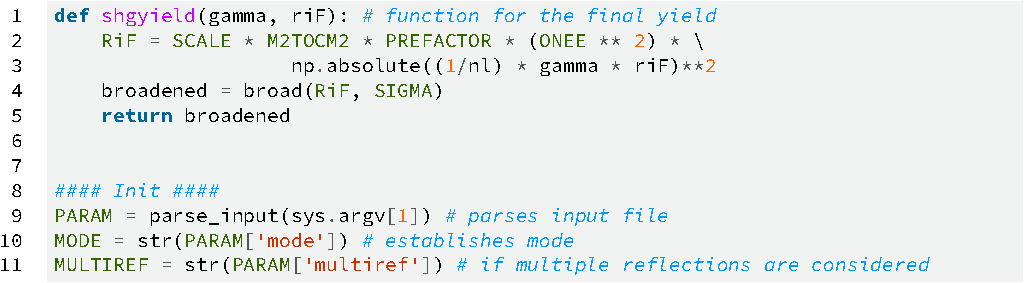
\includegraphics[width=\textwidth]{code-shgyield}
\end{figure}
https://github.com/roguephysicist/SHGYield
\end{frame}

\end{document}
